% Complete translation draft of Chapter 2; source PDF pages 18--49.
% Local symbols and styles used only by this chapter.
\providecommand{\ctsmiley}{\mathord{\tikz[baseline=-.5ex,x=.7ex,y=.7ex]{\draw (0,0) circle (1);\fill (-.35,.3) circle (.09);\fill (.35,.3) circle (.09);\draw (-.5,-.15) arc[start angle=210,end angle=330,radius=.58];}}}
\providecommand{\cttype}[1]{\(\ulcorner\)#1\(\urcorner\)}
\tikzset{cttwo/.style={draw,align=center,font=\small,inner sep=5pt},ctarrow/.style={-{Stealth[length=2mm]},font=\footnotesize},ctlabel/.style={font=\footnotesize,align=center,fill=white,inner sep=2pt}}
% Source: printed p. 9; PDF p. 18
\chapter{Phạm trù các tập hợp}
Lý thuyết tập hợp được xây dựng để làm nền tảng cho toàn bộ toán học. Các khái niệm tập hợp và hàm là cơ sở để hình thành trực giác về phạm trù nói chung. Chương này đưa ra các ví dụ về tập hợp và hàm, rồi bàn về biểu đồ giao hoán. Sau đó, chúng ta giới thiệu olog, qua đó dùng ngôn ngữ của lý thuyết phạm trù để nói về những khái niệm trong thế giới thực. Tất cả nội dung này thuộc lý thuyết tập hợp cơ bản, nhưng cũng có thể xem là một khảo sát về \emph{phạm trù các tập hợp}, ký hiệu là $\mathbf{Set}$.
\section{Tập hợp và hàm}
Từ lâu, con người đã thấy việc đặt các vật vào những ngăn chứa là hữu ích.
\begin{center}\begin{tikzpicture}
\node[cttwo] (a) {một vật};\node[cttwo,right=3cm of a] (b) {một ngăn chứa};\draw[ctarrow] (a)--node[above,ctlabel]{được đặt vào}(b);
\end{tikzpicture}\end{center}
Nghiên cứu tập hợp là nghiên cứu các vật trong những ngăn chứa.
\subsection{Tập hợp}
Có lẽ bạn đã có một hiểu biết trực giác về tập hợp. Ta có thể xem một tập hợp $X$ là một bộ sưu tập các \emph{phần tử} $x\in X$, trong đó nhận biết được mỗi phần tử là thuộc $X$, và với mỗi cặp phần tử đã được đặt tên $x,x'\in X$, ta có thể xác định liệu $x=x'$ hay không.\footnote{Ký hiệu $x'$, đọc là ``x phẩy'', không liên quan đến giải tích hay đạo hàm. Nó chỉ là ký hiệu dùng để đặt tên cho một đối tượng có nét tương tự $x$. Sự gợi ý về mối liên hệ giữa $x$ và $x'$ chỉ nhằm hỗ trợ nhận thức của con người, không phải là một phần của nội dung toán học.} Tập hợp các con lắc là bộ sưu tập những vật mà chúng ta thống nhất gọi là con lắc, mỗi vật đều
% Source: printed p. 10; PDF p. 19
được nhận biết là một con lắc, và khi hai người chỉ vào các con lắc, ta có thể xác định họ có đang chỉ vào cùng một con lắc hay không.
\begin{figure}[htbp]\centering
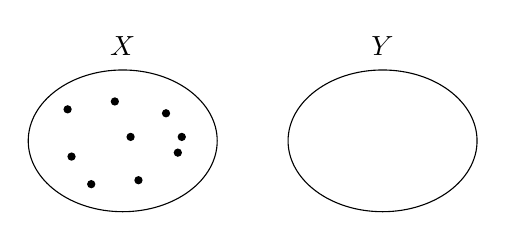
\begin{tikzpicture}[x=1cm,y=1cm]
\draw (0,0) ellipse (1.2 and .9);\node at (0,1.2){$X$};
\foreach \x/\y in {-.7/.4,-.1/.5,.55/.35,-.65/-.2,.1/.05,.7/-.15,-.4/-.55,.2/-.5,.75/.05}{\fill (\x,\y) circle (1.5pt);}
\draw (3.3,0) ellipse (1.2 and .9);\node at (3.3,1.2){$Y$};
\end{tikzpicture}
\caption{Một tập hợp $X$ có chín phần tử, và một tập hợp $Y$ không có phần tử nào, $Y=\varnothing$.}\label{fig:2-1}
\end{figure}
\paragraph{Ký hiệu 2.1.1.1.} Ký hiệu $\varnothing$ biểu thị tập hợp không có phần tử nào (xem Hình 2.1); ta cũng có thể viết tập hợp đó là $\{\}$. Ký hiệu $\mathbb N$ biểu thị tập hợp các số tự nhiên:
\begin{equation*}\mathbb N:=\{0,1,2,3,4,\ldots,877,\ldots\}.\tag{2.1}\end{equation*}
Ký hiệu $\mathbb Z$ biểu thị tập hợp các số nguyên, chứa cả các số tự nhiên lẫn các số đối của chúng,
\begin{equation*}\mathbb Z:=\{\ldots,-551,\ldots,-2,-1,0,1,2,\ldots\}.\tag{2.2}\end{equation*}
Nếu $A$ và $B$ là các tập hợp, ta nói $A$ là một \emph{tập con} của $B$, và viết $A\subseteq B$, nếu mỗi phần tử của $A$ là một phần tử của $B$. Do đó $\mathbb N\subseteq\mathbb Z$. Kiểm tra định nghĩa, ta thấy với mọi tập hợp $A$, ta có các tập con (có lẽ không thú vị lắm) $\varnothing\subseteq A$ và $A\subseteq A$. Ta có thể dùng \emph{ký hiệu mô tả tập hợp bằng điều kiện} để biểu thị các tập con. Chẳng hạn, tập hợp các số nguyên chẵn có thể viết là $\{n\in\mathbb Z\mid n\text{ chẵn}\}$. Tập hợp các số nguyên lớn hơn 2 có thể viết theo nhiều cách, chẳng hạn
\[\{n\in\mathbb Z\mid n>2\}\quad\text{hoặc}\quad\{n\in\mathbb N\mid n>2\}\quad\text{hoặc}\quad\{n\in\mathbb N\mid n\geq3\}.\]
Ký hiệu $\exists$ nghĩa là ``tồn tại''. Vì thế, ta có thể viết tập hợp các số nguyên chẵn là
\[\{n\in\mathbb Z\mid n\text{ chẵn}\}=\{n\in\mathbb Z\mid\exists m\in\mathbb Z\text{ sao cho }2m=n\}.\]
Ký hiệu $\exists!$ nghĩa là ``tồn tại duy nhất''. Do đó, phát biểu ``$\exists!x\in\mathbb R$ sao cho $x^2=0$'' nghĩa là có một và chỉ một số có bình phương bằng 0. Cuối cùng, ký hiệu $\forall$
% Source: printed p. 11; PDF p. 20
nghĩa là ``với mọi''. Vì thế, phát biểu ``$\forall m\in\mathbb N\ \exists n\in\mathbb N$ sao cho $m<n$'' nghĩa là với mỗi số đều có một số lớn hơn.

Như bạn có thể đã nhận thấy khi định nghĩa $\mathbb N$ và $\mathbb Z$ trong (2.1) và (2.2), ta dùng ký hiệu hai chấm bằng ``$A:=XYZ$'' với nghĩa đại loại là ``định nghĩa $A$ là $XYZ$''. Tức là, một tuyên bố dùng dấu hai chấm bằng không biểu thị một sự thật tự nhiên (như $2+2=4$), mà biểu thị một lựa chọn của người viết.

Ta cũng thường bàn về một tập hợp cụ thể có một phần tử, ký hiệu $\{\ctsmiley\}$, cũng như tập hợp quen thuộc các số thực $\mathbb R$ và một số biến thể, chẳng hạn $\mathbb R_{\geq0}:=\{x\in\mathbb R\mid x\geq0\}$.
\paragraph{Bài tập 2.1.1.2.} Cho $A:=\{1,2,3\}$. Tất cả các tập con của $A$ là những tập nào? Gợi ý: Có tám tập.\hfill$\diamond$
\paragraph{Lời giải 2.1.1.2.} Sáu tập dễ thấy nhất là:
\[\{1\},\quad\{2\},\quad\{3\},\quad\{1,2\},\quad\{1,3\},\quad\{2,3\}.\]
Nhưng tập rỗng và toàn bộ tập hợp cũng luôn là các tập con:
\[\varnothing,\quad\{1,2,3\}.\]\hfill$\diamond$

Một tập hợp có thể có các tập hợp khác làm phần tử. Chẳng hạn, tập hợp
\[X:=\{\{1,2\},\{4\},\{1,3,6\}\}\]
có ba phần tử, mỗi phần tử là một tập hợp.
\subsection{Hàm}
Nếu $X$ và $Y$ là các tập hợp, thì một \emph{hàm $f$ từ $X$ đến $Y$}, ký hiệu $f:X\to Y$, là một ánh xạ gửi mỗi phần tử $x\in X$ đến một phần tử của $Y$, ký hiệu $f(x)\in Y$. Ta gọi $X$ là \emph{miền xác định} của hàm $f$, và gọi $Y$ là \emph{đối miền} của $f$.

Lưu ý rằng với mỗi phần tử $x\in X$, có đúng một mũi tên xuất phát từ $x$, nhưng với một phần tử $y\in Y$, có thể có nhiều mũi tên chỉ đến $y$, hoặc không có mũi tên nào chỉ đến $y$ (xem Hình 2.2).
\paragraph{Cách nói gợi nhớ 2.1.2.1.}
Cho một hàm $f:X\to Y$. Ta xem $X$ là một tập hợp các vật, còn $Y$ là một tập hợp các ngăn chứa. Hàm cho biết phải đặt mỗi vật vào ngăn nào.
% Source: printed p. 12; PDF p. 21
\begin{figure}[htbp]\centering
\begin{tikzpicture}[x=1cm,y=.75cm]
\draw (0,-1.5) ellipse (1 and 2.2);\draw (4,-2) ellipse (1.1 and 2.4);
\node at (0,1.05){$X$};\node at (4,1.05){$Y$};
\foreach \i in {1,...,4}{\coordinate (x\i) at (0,{1-\i});\fill (x\i) circle (1.2pt);\node[left,font=\small] at (x\i){$x_{\i}$};}
\foreach \i in {1,...,5}{\coordinate (y\i) at (4,{1-\i});\fill (y\i) circle (1.2pt);\node[right,font=\small] at (y\i){$y_{\i}$};}
\draw[ctarrow] (x1)--(y1);\draw[ctarrow] (x2)--(y2);\draw[ctarrow] (x3)--(y4);\draw[ctarrow] (x4)--(y1);
\end{tikzpicture}
\caption{Một hàm từ tập hợp $X$ đến tập hợp $Y$.}\label{fig:2-2}
\end{figure}
\paragraph{Ứng dụng 2.1.2.2.} Khi nghiên cứu cơ học vật liệu, người ta muốn biết một vật liệu phản ứng ra sao trước lực kéo. Chẳng hạn, một dây cao su phản ứng với lực kéo khác với một lò xo. Với mỗi vật liệu, ta có thể gắn một đường cong lực--độ giãn, ghi lại lực mà vật liệu chịu khi được kéo giãn đến những độ dài khác nhau. Khi đã cố định một phương pháp tiến hành thí nghiệm, việc tìm đường cong lực--độ giãn của một vật liệu, trong điều kiện lý tưởng, sẽ tạo thành một hàm từ tập hợp các vật liệu đến tập hợp các đường cong.\hfill$\diamond\diamond$
\paragraph{Bài tập 2.1.2.3.} Sau đây là một mô tả giản lược về cách bộ não tiếp nhận ánh sáng. Mắt chứa khoảng 100 triệu tế bào thụ cảm ánh sáng (PR). Mỗi tế bào này nối với một tế bào hạch võng mạc (RG). Không có tế bào PR nào nối với hai tế bào RG khác nhau, nhưng thường nhiều tế bào PR có thể nối với cùng một tế bào RG.

Gọi $PR$ là tập hợp các tế bào thụ cảm ánh sáng, và $RG$ là tập hợp các tế bào hạch võng mạc.
\begin{enumerate}[label=\alph*.]
\item Theo mô tả trên, kiểu kết nối này tạo thành một hàm $RG\to PR$, một hàm $PR\to RG$, hay không tạo thành hàm nào trong hai hàm đó?
\item Bạn có đoán rằng những kiểu kết nối giữa các vùng khác của bộ não có dạng hàm hay không? Hãy giải thích câu trả lời.
\end{enumerate}\hfill$\diamond$
% Source: printed p. 13; PDF p. 22
\paragraph{Lời giải 2.1.2.3.}
\begin{enumerate}[label=\alph*.]
\item Với mỗi phần tử của $PR$, ta gắn một phần tử của $RG$, nên đây là một hàm $PR\to RG$.
\item (Mọi phỏng đoán có giải thích đều chấp nhận được.) Không có kiến thức nền về chủ đề này, tôi có thể đoán rằng điều đó xảy ra trong mọi trường hợp tri giác trực tiếp được chuyển thành các xung thần kinh.
\end{enumerate}\hfill$\diamond$
\paragraph{Ví dụ 2.1.2.4.} Giả sử $X$ là một tập hợp và $X'\subseteq X$ là một tập con. Khi đó, ta có thể xét hàm $X'\to X$ gửi mỗi phần tử của $X'$ đến ``chính nó'' khi được xem là phần tử của $X$. Chẳng hạn, nếu $X=\{a,b,c,d,e,f\}$ và $X'=\{b,d,e\}$, thì $X'\subseteq X$. Ta biến điều này thành hàm $X'\to X$ được cho bởi $b\mapsto b$, $d\mapsto d$, $e\mapsto e$.\footnote{Loại mũi tên này, $\mapsto$, được đọc là ``được ánh xạ đến''. Một hàm $f:X\to Y$ là một quy tắc gán cho mỗi phần tử $x\in X$ một phần tử $f(x)\in Y$. Ta nói ``$x$ được ánh xạ đến $f(x)$'' và viết $x\mapsto f(x)$.}

Về mặt ký hiệu, đôi khi ta có thể nói như sau: Cho $X$ là một tập hợp, và cho $i:X'\subseteq X$ là một tập con. Ở đây ta làm rõ rằng $X'$ là một tập con của $X$, còn $i$ là tên của hàm tương ứng.
\paragraph{Bài tập 2.1.2.5.} Cho $f:\mathbb N\to\mathbb N$ là hàm gửi mỗi số tự nhiên đến bình phương của nó, chẳng hạn $f(6)=36$. Trước hết hãy điền vào chỗ trống, rồi trả lời câu hỏi.
\begin{enumerate}[label=\alph*.]
\item $2\mapsto\underline{\hspace{1cm}}$
\item $0\mapsto\underline{\hspace{1cm}}$
\item $-2\mapsto\underline{\hspace{1cm}}$
\item $5\mapsto\underline{\hspace{1cm}}$
\item Xét hai ký hiệu $\to$ và $\mapsto$. Cách dùng hai ký hiệu này từ đầu sách đến đây khác nhau như thế nào?
\end{enumerate}\hfill$\diamond$
\paragraph{Lời giải 2.1.2.5.}
\begin{enumerate}[label=\alph*.]
\item 4.
\item 0.
\item Hàm không áp dụng cho $-2$, vì $-2$ không phải là một phần tử của $\mathbb N$.
% Source: printed p. 14; PDF p. 23
\item 25.
\item Ký hiệu $\to$ dùng để biểu thị một hàm từ tập hợp này đến tập hợp khác. Chẳng hạn, mũi tên trong $g:X\to Y$ là một ký hiệu cho biết $g$ là tên của một hàm từ tập hợp $X$ đến tập hợp $Y$. Ký hiệu $\mapsto$ dùng để cho biết hàm gửi một phần tử cụ thể của miền xác định đến đâu. Vì thế, với hàm bình phương $f:\mathbb N\to\mathbb N$, ta viết $5\mapsto25$ vì hàm $f$ gửi 5 đến 25.
\end{enumerate}\hfill$\diamond$

Cho một hàm $f:X\to Y$. Các phần tử của $Y$ mà có ít nhất một mũi tên chỉ đến được gọi là thuộc \emph{ảnh} của $f$; tức là
\begin{equation*}\operatorname{im}(f):=\{y\in Y\mid\exists x\in X\text{ sao cho }f(x)=y\}.\tag{2.3}\end{equation*}
Ảnh của một hàm $f$ luôn là một tập con của đối miền của nó, $\operatorname{im}(f)\subseteq Y$.
\paragraph{Bài tập 2.1.2.6.} Nếu hàm $f:X\to Y$ được biểu diễn trong Hình 2.2, hãy viết ảnh của nó, $\operatorname{im}(f)$, dưới dạng một tập hợp.\hfill$\diamond$
\paragraph{Lời giải 2.1.2.6.} Ảnh là $\operatorname{im}(f)=\{y_1,y_2,y_4\}$.\hfill$\diamond$

Cho một hàm $f:X\to Y$ và một hàm $g:Y\to Z$, trong đó đối miền của $f$ chính là miền xác định của $g$ (cùng là $Y$), ta nói $f$ và $g$ \emph{có thể hợp thành}:
\[X\xrightarrow{f}Y\xrightarrow{g}Z.\]
\emph{Hợp thành} của $f$ và $g$ được ký hiệu là $g\circ f:X\to Z$. Xem Hình 2.3.
\paragraph{Cách nói gợi nhớ 2.1.2.7.} Cho các hàm có thể hợp thành $X\xrightarrow{f}Y\xrightarrow{g}Z$. Ta có một cách đặt mỗi vật trong $X$ vào một ngăn chứa trong $Y$, và một cách đặt mỗi ngăn chứa trong $Y$ vào một ngăn chứa lớn hơn trong $Z$. Hàm hợp thành $g\circ f:X\to Z$ là cách thu được để đặt mỗi vật trong $X$ vào một ngăn chứa trong $Z$.
\paragraph{Bài tập 2.1.2.8.} Nếu $A\subseteq X$ là một tập con, Ví dụ 2.1.2.4 đã cho thấy cách xem nó là một hàm $i:A\to X$. Cho một hàm $f:X\to Y$, ta có thể hợp thành $A\xrightarrow{i}X\xrightarrow{f}Y$ và thu được một hàm $f\circ i:A\to Y$. Ảnh của hàm này được ký hiệu
\[f(A):=\operatorname{im}(f\circ i),\]
% Source: printed p. 15; PDF p. 24
xem (2.3) để biết định nghĩa của ảnh.
\begin{figure}[htbp]\centering
\begin{tikzpicture}[x=1cm,y=.65cm]
\foreach \x/\n/\h in {0/X/1.7,3/Y/2.3,6/Z/1.2}{\draw (\x,-1) ellipse (1 and \h);\node at (\x,{\h-.5}){$\n$};}
\foreach \i in {1,2,3}{\coordinate (x\i) at (0,{1-\i});\fill (x\i) circle (1.2pt);\node[left,font=\small] at (x\i){$x_{\i}$};}
\foreach \i in {1,2,3,4}{\coordinate (y\i) at (3,{1.5-\i});\fill (y\i) circle (1.2pt);\node[above=1pt,inner sep=0pt,font=\small] at (y\i){$y_{\i}$};}
\foreach \i in {1,2}{\coordinate (z\i) at (6,{.5-\i});\fill (z\i) circle (1.2pt);\node[right,font=\small] at (z\i){$z_{\i}$};}
\draw[ctarrow] (x1)--(y1);\draw[ctarrow] (x2)--(y2);\draw[ctarrow] (x3)--(y4);
\draw[ctarrow] (y1)--(z1);\draw[ctarrow] (y2)--(z2);\draw[ctarrow] (y3)--(z1);\draw[ctarrow] (y4)--(z2);
\end{tikzpicture}
\caption{Các hàm $f:X\to Y$ và $g:Y\to Z$ hợp thành một hàm $g\circ f:X\to Z$ (hãy đi theo các mũi tên).}\label{fig:2-3}
\end{figure}
Cho $X=Y:=\mathbb Z$, $A:=\{-1,0,1,2,3\}\subseteq X$, và $f:X\to Y$ được cho bởi $f(x)=x^2$. Tập ảnh $f(A)$ là gì?\hfill$\diamond$
\paragraph{Lời giải 2.1.2.8.} Theo định nghĩa của ảnh (xem (2.3)), ta có
\[f(A)=\{y\in\mathbb Z\mid\exists a\in A\text{ sao cho }f\circ i(a)=y\}.\]
Vì $A=\{-1,0,1,2,3\}$ và $i(a)=a$ với mọi $a\in A$, nên $f(A)=\{0,1,4,9\}$. Lưu ý rằng một phần tử của một tập hợp chỉ có thể xuất hiện trong tập hợp ấy một lần; mặc dù $f(-1)=f(1)=1$, ta chỉ cần nêu 1 một lần trong $f(A)$. Nói cách khác, nếu một sinh viên đưa ra đáp án như $\{1,0,1,4,9\}$, điều này gợi ý một sự nhầm lẫn nhỏ.\hfill$\diamond$
\paragraph{Ký hiệu 2.1.2.9.} Cho $X$ là một tập hợp và $x\in X$ là một phần tử. Có một hàm $\{\ctsmiley\}\to X$ gửi $\ctsmiley\mapsto x$. Ta nói hàm này \emph{biểu diễn} $x\in X$. Ta có thể ký hiệu nó là $x:\{\ctsmiley\}\to X$.
% Source: printed p. 16; PDF p. 25
\paragraph{Bài tập 2.1.2.10.} Cho $X$ là một tập hợp, $x\in X$ là một phần tử, và $x:\{\ctsmiley\}\to X$ là hàm biểu diễn phần tử đó. Với một hàm $f:X\to Y$, $f\circ x$ là gì?\hfill$\diamond$
\paragraph{Lời giải 2.1.2.10.} Đó là hàm $\{\ctsmiley\}\to Y$ gửi $\ctsmiley$ đến $f(x)$. Nói cách khác, nó biểu diễn phần tử $f(x)$.\hfill$\diamond$
\paragraph{Nhận xét 2.1.2.11.} Giả sử cho các tập hợp $A,B,C$ và các hàm $A\xrightarrow{f}B\xrightarrow{g}C$. Từ đầu đến đây, ta đã dùng thứ tự cổ điển để viết hợp thành của chúng, tức là $g\circ f:A\to C$. Với mỗi phần tử $a\in A$, ta viết $g\circ f(a)$ để chỉ $g(f(a))$. Điều này nghĩa là ``thực hiện $g$ trên kết quả của việc thực hiện $f$ trên $a$''.

Tuy nhiên, có một cách khác để viết hợp thành này, gọi là \emph{thứ tự biểu đồ}. Thay vì $g\circ f$, ta viết $f;g:A\to C$, nghĩa là ``thực hiện $f$, rồi thực hiện $g$''. Cho một phần tử $a\in A$, được biểu diễn bởi $a:\{\ctsmiley\}\to A$, ta có một phần tử $a;f;g$.

Cho $X$ và $Y$ là các tập hợp. Ta viết $\operatorname{Hom}_{\mathbf{Set}}(X,Y)$ để biểu thị tập hợp các hàm $X\to Y$.\footnote{Ký hiệu $\operatorname{Hom}_{\mathbf{Set}}(-,-)$ sẽ trở nên dễ hiểu hơn khi được đặt trong một bối cảnh rộng hơn về sau. Đặc biệt, xem Mục 5.1.} Lưu ý rằng hai hàm $f,g:X\to Y$ bằng nhau khi và chỉ khi với mỗi phần tử $x\in X$, ta có $f(x)=g(x)$.
\paragraph{Bài tập 2.1.2.12.} Cho $A=\{1,2,3,4,5\}$ và $B=\{x,y\}$.
\begin{enumerate}[label=\alph*.]\item $\operatorname{Hom}_{\mathbf{Set}}(A,B)$ có bao nhiêu phần tử?\item $\operatorname{Hom}_{\mathbf{Set}}(B,A)$ có bao nhiêu phần tử?\end{enumerate}\hfill$\diamond$
\paragraph{Lời giải 2.1.2.12.}
\begin{enumerate}[label=\alph*.]\item 32. Chẳng hạn, $1\mapsto x$, $2\mapsto x$, $3\mapsto x$, $4\mapsto y$, $5\mapsto x$.\item 25. Chẳng hạn, $x\mapsto1$, $y\mapsto4$.\end{enumerate}\hfill$\diamond$
% Source: printed p. 17; PDF p. 26
\paragraph{Bài tập 2.1.2.13.}
\begin{enumerate}[label=\alph*.]
\item Tìm một tập hợp $A$ sao cho với mọi tập hợp $X$, có đúng một phần tử trong $\operatorname{Hom}_{\mathbf{Set}}(X,A)$. Gợi ý: Vẽ hình cho những tập $A$ và $X$ mà bạn đề xuất. $A$ nên có bao nhiêu chấm?
\item Tìm một tập hợp $B$ sao cho với mọi tập hợp $X$, có đúng một phần tử trong $\operatorname{Hom}_{\mathbf{Set}}(B,X)$.
\end{enumerate}\hfill$\diamond$
\paragraph{Lời giải 2.1.2.13.}
\begin{enumerate}[label=\alph*.]
\item Đây là một tập như vậy: $A:=\{\ctsmiley\}$. (Một tập khác là $A:=\{48\}$, và một tập khác nữa là $A:=\{a_1\}$.)
\begin{center}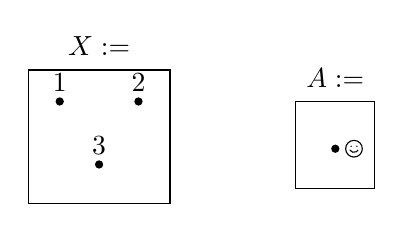
\begin{tikzpicture}
\draw (-.9,-.7) rectangle (.9,1);\node at (0,1.3){$X:=$};\draw (2.5,-.5) rectangle (3.5,.6);\node at (3,.9){$A:=$};
\foreach \i/\x/\y in {1/-.5/.6,2/.5/.6,3/0/-.2}{\fill (\x,\y) circle (1.5pt);\node[above] at (\x,\y){$\i$};}
\fill (3,0) circle (1.5pt);\node[right] at (3,0){$\ctsmiley$};
\end{tikzpicture}\end{center}
Tại sao? Ta đang cố đếm số hàm $X\to A$. Bất kể $X$ và $A$ là gì, để cho một hàm $X\to A$, ta phải trả lời nhiều lần câu hỏi ``Tôi gửi $x$ đến đâu?'', một lần cho mỗi phần tử $x\in X$. Mỗi phần tử của $X$ được gửi đến một phần tử của $A$. Chẳng hạn, nếu $X=\{1,2,3\}$, ta đặt ba câu hỏi: Tôi gửi 1 đến đâu? Tôi gửi 2 đến đâu? Tôi gửi 3 đến đâu? Khi $A$ chỉ có một phần tử, chỉ có một nơi để gửi mỗi $x$. Một hàm $X\to\{\ctsmiley\}$ được viết là $1\mapsto\ctsmiley$, $2\mapsto\ctsmiley$, $3\mapsto\ctsmiley$. Chỉ có một hàm như vậy, nên $\operatorname{Hom}_{\mathbf{Set}}(X,\{\ctsmiley\})$ có một phần tử.
\item $B=\varnothing$ là khả năng duy nhất.
\begin{center}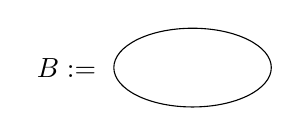
\begin{tikzpicture}\draw (0,0) ellipse (1 and .5);\node[left] at (-1.1,0){$B:=$};\end{tikzpicture}\end{center}
Để cho một hàm $B\to X$, ta phải trả lời câu hỏi ``Tôi gửi $b$ đến đâu?'' với mỗi $b\in B$. Vì $B$ không có phần tử, ta không phải trả lời câu hỏi nào để cho một hàm như thế. Có một cách trả lời tất cả các câu hỏi cần thiết, vì việc đó được hoàn thành ngay lập tức (``thỏa mãn một cách hiển nhiên khi không có trường hợp nào cần xét''). Điều này giống như yêu cầu John ``gán một điểm chữ cho mỗi người cao hơn 14 foot''. John hoàn thành việc ngay khi nhận được yêu cầu, và chỉ có một cách để anh ấy hoàn thành việc đó. Vì vậy, $\operatorname{Hom}_{\mathbf{Set}}(\varnothing,X)$ có một phần tử.\nobreak\hfill$\diamond$
\end{enumerate}
% Source: printed p. 18; PDF p. 27
\begin{figure}[htbp]\centering
\begin{tikzpicture}[x=1cm,y=.7cm]
\draw (0,-1.5) ellipse (1 and 2);\draw (4,-1.5) ellipse (1 and 2);\node at (0,.9){$X$};\node at (4,.9){$Y$};
\foreach \i in {1,...,4}{\coordinate (x\i) at (0,{1-\i});\fill (x\i) circle (1.2pt);\node[left,font=\small] at (x\i){$x_{\i}$};\coordinate (y\i) at (4,{1-\i});\fill (y\i) circle (1.2pt);\node[right,font=\small] at (y\i){$y_{\i}$};}
\draw[ctarrow] (x1)--(y1);\draw[ctarrow] (x2)--(y3);\draw[ctarrow] (x3)--(y4);\draw[ctarrow] (x4)--(y2);
\end{tikzpicture}
\caption{Một đẳng cấu $X\xrightarrow{\cong}Y$.}\label{fig:2-4}
\end{figure}
Với mọi tập hợp $X$, ta định nghĩa \emph{hàm đồng nhất} trên $X$, ký hiệu
\[\operatorname{id}_X:X\to X,\]
là hàm sao cho với mọi $x\in X$, ta có $\operatorname{id}_X(x)=x$.
\paragraph{Định nghĩa 2.1.2.14 (Đẳng cấu).} Cho $X$ và $Y$ là các tập hợp. Một hàm $f:X\to Y$ được gọi là một \emph{đẳng cấu}, ký hiệu $f:X\xrightarrow{\cong}Y$, nếu tồn tại một hàm $g:Y\to X$ sao cho $g\circ f=\operatorname{id}_X$ và $f\circ g=\operatorname{id}_Y$.
\[\begin{tikzcd}X\arrow[r,bend left=25,"f"]&Y\arrow[l,bend left=25,"g"]\end{tikzcd}\]
Trong trường hợp này, ta cũng nói $f$ là \emph{khả nghịch} và $g$ là \emph{nghịch đảo} của $f$. Nếu tồn tại một đẳng cấu $X\xrightarrow{\cong}Y$, ta nói $X$ và $Y$ là các \emph{tập hợp đẳng cấu} và có thể viết $X\cong Y$.
\paragraph{Ví dụ 2.1.2.15.} Nếu $X$ và $Y$ là các tập hợp, và $f:X\to Y$ là một đẳng cấu, thì hình tương tự Hình 2.2 sẽ trông như một phép ghép cặp hoàn hảo, thường được gọi là một \emph{tương ứng một-một}. Điều đó nghĩa là không có hai mũi tên nào cùng chỉ đến một phần tử của $Y$, và mọi phần tử của $Y$ đều thuộc ảnh. Chẳng hạn, Hình 2.4 biểu diễn một đẳng cấu $X\xrightarrow{\cong}Y$ giữa hai tập hợp có bốn phần tử.
% Source: printed p. 19; PDF p. 28
\paragraph{Ứng dụng 2.1.2.16.} Có một đẳng cấu giữa tập hợp $\mathrm{Nuc}_{\mathrm{DNA}}$ các nucleotide có trong DNA và tập hợp $\mathrm{Nuc}_{\mathrm{RNA}}$ các nucleotide có trong RNA. Thật vậy, cả hai tập hợp đều có bốn phần tử, nên có 24 đẳng cấu khác nhau. Nhưng chỉ có một đẳng cấu hữu ích trong sinh học. Trước khi nêu đẳng cấu đó, hãy lưu ý rằng còn có một đẳng cấu $\mathrm{Nuc}_{\mathrm{DNA}}\cong\{A,C,G,T\}$ và một đẳng cấu $\mathrm{Nuc}_{\mathrm{RNA}}\cong\{A,C,G,U\}$; ta sẽ dùng các chữ cái để viết tắt tên các nucleotide.

Đẳng cấu tiện dụng $\mathrm{Nuc}_{\mathrm{DNA}}\xrightarrow{\cong}\mathrm{Nuc}_{\mathrm{RNA}}$ được cho bởi quá trình phiên mã RNA; nó gửi
\[A\mapsto U,\quad C\mapsto G,\quad G\mapsto C,\quad T\mapsto A.\]
(Xem thêm Ứng dụng 5.1.2.21.) Cũng có một đẳng cấu $\mathrm{Nuc}_{\mathrm{DNA}}\xrightarrow{\cong}\mathrm{Nuc}_{\mathrm{DNA}}$ (sự ghép cặp trong chuỗi xoắn kép), được cho bởi
\[A\mapsto T,\quad C\mapsto G,\quad G\mapsto C,\quad T\mapsto A.\]
Quá trình sản xuất protein có thể được mô hình hóa bằng một hàm từ tập hợp các chuỗi gồm 3 nucleotide đến tập hợp các amino acid của sinh vật nhân thực. Tuy nhiên, hàm này không thể là một đẳng cấu, vì có $4^3=64$ bộ ba nucleotide RNA nhưng chỉ có 21 amino acid của sinh vật nhân thực.\hfill$\diamond\diamond$
\paragraph{Bài tập 2.1.2.17.} Cho $n\in\mathbb N$ là một số tự nhiên, và $X$ là một tập hợp có đúng $n$ phần tử.
\begin{enumerate}[label=\alph*.]\item Có bao nhiêu đẳng cấu từ $X$ đến chính nó?\item Công thức của bạn trong phần (a) có đúng khi $n=0$ không?\end{enumerate}\hfill$\diamond$
\paragraph{Lời giải 2.1.2.17.}
\begin{enumerate}[label=\alph*.]
\item Có $n!$, đọc là ``$n$ giai thừa''. Chẳng hạn, nếu $X=\{a,b,c,d\}$, thì ta có $4!=4*3*2*1=24$ đẳng cấu $X\xrightarrow{\cong}X$. Một đẳng cấu như vậy là $a\mapsto a$, $b\mapsto d$, $c\mapsto b$, $d\mapsto c$.\begingroup\renewcommand{\thefootnote}{*}\footnote[0]{Chú thích của người dịch: Bản gốc in $d\mapsto b$. Ở đây sửa thành $d\mapsto c$, vì nếu cả $c$ lẫn $d$ đều được gửi đến $b$, hàm sẽ không phải là một tương ứng một-một.}\endgroup
 Lý do trực giác khiến đáp án là $4!$ là: có bốn cách chọn nơi gửi $a$ đến, nhưng sau đó chỉ còn ba cách chọn nơi gửi $b$ đến, rồi chỉ còn hai cách chọn nơi gửi $c$ đến, và cuối cùng chỉ còn một cách chọn nơi gửi $d$ đến. Để thực sự hiểu đáp án này, hãy tự liệt kê mọi đẳng cấu $\{1,2,3,4\}\xrightarrow{\cong}\{1,2,3,4\}$.
\item Có, có một hàm $\varnothing\to\varnothing$ và nó là một đẳng cấu.
\end{enumerate}\hfill$\diamond$
% Source: printed p. 20; PDF p. 29
\paragraph{Mệnh đề 2.1.2.18.} Các sự kiện sau đúng đối với đẳng cấu.
\begin{enumerate}
\item Mọi tập hợp $A$ đều đẳng cấu với chính nó; tức là tồn tại một đẳng cấu $A\xrightarrow{\cong}A$.
\item Với mọi tập hợp $A$ và $B$, nếu $A$ đẳng cấu với $B$, thì $B$ đẳng cấu với $A$.
\item Với mọi tập hợp $A,B,C$, nếu $A$ đẳng cấu với $B$ và $B$ đẳng cấu với $C$, thì $A$ đẳng cấu với $C$.
\end{enumerate}
\begin{proof}
\begin{enumerate}
\item Hàm đồng nhất $\operatorname{id}_A:A\to A$ là khả nghịch; nghịch đảo của nó là $\operatorname{id}_A$, vì $\operatorname{id}_A\circ\operatorname{id}_A=\operatorname{id}_A$.
\item Nếu $f:A\to B$ là khả nghịch với nghịch đảo $g:B\to A$, thì $g$ là một đẳng cấu với nghịch đảo $f$.
\item Nếu $f:A\to B$ và $f':B\to C$ đều khả nghịch với các nghịch đảo $g:B\to A$ và $g':C\to B$, thì các phép tính sau cho thấy $f'\circ f$ khả nghịch với nghịch đảo $g\circ g'$:
\begin{align*}
(f'\circ f)\circ(g\circ g')&=f'\circ(f\circ g)\circ g'=f'\circ\operatorname{id}_B\circ g'=f'\circ g'=\operatorname{id}_C,\\
(g\circ g')\circ(f'\circ f)&=g\circ(g'\circ f')\circ f=g\circ\operatorname{id}_B\circ f=g\circ f=\operatorname{id}_A.
\end{align*}
\end{enumerate}
\end{proof}
\paragraph{Bài tập 2.1.2.19.} Cho $A$ và $B$ là các tập hợp sau:
\begin{center}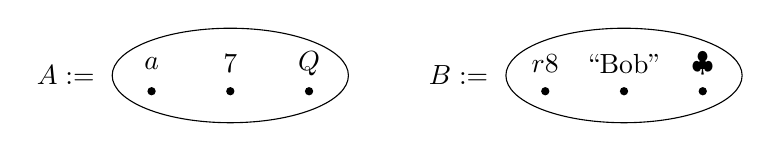
\begin{tikzpicture}[x=1cm]
\draw (0,0) ellipse (1.5 and .6);\node[left] at (-1.6,0){$A:=$};
\foreach \x/\s in {-1/a,0/7,1/Q}{\fill (\x,-.2) circle (1.5pt);\node at (\x,.15){$\s$};}
\draw (5,0) ellipse (1.5 and .6);\node[left] at (3.4,0){$B:=$};\fill (4,-.2) circle (1.5pt);\fill (5,-.2) circle (1.5pt);\fill (6,-.2) circle (1.5pt);\node at (4,.15){$r8$};\node at (5,.15){``Bob''};\node at (6,.15){$\clubsuit$};
\end{tikzpicture}\end{center}
Lưu ý rằng các tập hợp $A$ và $B$ đẳng cấu. Giả sử $f:B\to\{1,2,3,4,5\}$ gửi ``Bob'' đến 1, gửi $\clubsuit$ đến 3, và gửi $r8$ đến 4. Có một hàm \emph{chính tắc} $A\to\{1,2,3,4,5\}$ tương ứng với $f$ hay không?\footnote{``Chính tắc'', theo cách dùng ở đây, nghĩa đại loại là ``lựa chọn tốt nhất'', một lựa chọn nổi bật như lựa chọn hợp lý duy nhất.}\hfill$\diamond$
% Source: printed p. 21; PDF p. 30
\paragraph{Lời giải 2.1.2.19.} Không. Có nhiều lựa chọn, và không lựa chọn nào hợp lý hơn các lựa chọn khác, tức là không có lựa chọn nào chính tắc. (Thực ra có sáu lựa chọn; bạn có thấy tại sao không?)

Mục đích của bài tập này là minh họa rằng ngay cả khi biết hai tập hợp đẳng cấu, ta cũng không nhất thiết có thể xem chúng là như nhau. Để xem chúng là như nhau, ta cần có trong tay một đẳng cấu xác định $g:A\xrightarrow{\cong}B$, chẳng hạn $a\mapsto r8$, $7\mapsto\text{``Bob''}$, $Q\mapsto\clubsuit$. Khi đó, với $f:B\to\{1,2,3,4,5\}$, có một hàm chính tắc $A\to\{1,2,3,4,5\}$ tương ứng với $f$, chính là $f\circ g$.\hfill$\diamond$
\paragraph{Bài tập 2.1.2.20.} Tìm một tập hợp $A$ sao cho với mọi tập hợp $X$, có một đẳng cấu tập hợp
\[X\cong\operatorname{Hom}_{\mathbf{Set}}(A,X).\]
Gợi ý: Một hàm $A\to X$ chỉ mỗi phần tử của $A$ đến một phần tử của $X$. Khi nào số cách làm như vậy bằng số phần tử của $X$?\hfill$\diamond$
\paragraph{Lời giải 2.1.2.20.} Cho $A=\{\ctsmiley\}$. Khi đó, để chỉ mỗi phần tử của $A$ đến một phần tử của $X$, ta chỉ cần chỉ $\ctsmiley$ đến một phần tử của $X$. Tập hợp các cách làm như vậy có thể được đặt trong tương ứng một-một với tập hợp các phần tử của $X$. Chẳng hạn, nếu $X=\{1,2,3\}$, thì $\ctsmiley\mapsto3$ là một hàm $A\to X$ biểu diễn phần tử $3\in X$. Xem Ký hiệu 2.1.2.9.\hfill$\diamond$
\paragraph{Ký hiệu 2.1.2.21.} Với mỗi số tự nhiên $n\in\mathbb N$, định nghĩa một tập hợp
\begin{equation*}\underline n:=\{1,2,3,\ldots,n\}.\tag{2.4}\end{equation*}
Ta gọi $\underline n$ là \emph{tập hợp số hiệu} có kích thước $n$. Đặc biệt, $\underline2=\{1,2\}$, $\underline1=\{1\}$, và $\underline0=\varnothing$.

Cho $A$ là một tập hợp bất kỳ. Một hàm $f:\underline n\to A$ có thể viết thành một dãy độ dài $n$:
\begin{equation*}f=(f(1),f(2),\ldots,f(n)).\tag{2.5}\end{equation*}
Ta gọi đây là \emph{ký hiệu dãy} cho $f$.
\paragraph{Bài tập 2.1.2.22.}
\begin{enumerate}[label=\alph*.]
\item Cho $A=\{a,b,c,d\}$. Nếu $f:\underline{10}\to A$ được cho bằng ký hiệu dãy
\[(a,b,c,c,b,a,d,d,a,b),\]
thì $f(4)$ là gì?
\item Cho $s:\underline7\to\mathbb N$ được xác định bởi $s(i)=i^2$. Hãy viết $s$ bằng ký hiệu dãy.
\end{enumerate}\hfill$\diamond$
% Source: printed p. 22; PDF p. 31
\paragraph{Lời giải 2.1.2.22.}
\begin{enumerate}[label=\alph*.]\item $c$.\item $(1,4,9,16,25,36,49)$.\end{enumerate}\hfill$\diamond$
\paragraph{Định nghĩa 2.1.2.23 (Lực lượng của tập hợp hữu hạn).} Cho $A$ là một tập hợp và $n\in\mathbb N$ là một số tự nhiên. Ta nói $A$ có \emph{lực lượng} $n$, ký hiệu
\[|A|=n,\]
nếu tồn tại một đẳng cấu tập hợp $A\cong\underline n$. Nếu tồn tại một $n\in\mathbb N$ sao cho $A$ có lực lượng $n$, ta nói $A$ là \emph{hữu hạn}. Nếu không, ta nói $A$ là \emph{vô hạn} và viết $|A|\geq\infty$.
\paragraph{Bài tập 2.1.2.24.}
\begin{enumerate}[label=\alph*.]\item Cho $A=\{5,6,7\}$. $|A|$ là gì?\item $|\{1,1,2,3,5\}|$ là gì?\item $|\mathbb N|$ là gì?\item $|\{n\in\mathbb N\mid n\leq5\}|$ là gì?\end{enumerate}\hfill$\diamond$
\paragraph{Lời giải 2.1.2.24.}
\begin{enumerate}[label=\alph*.]
\item $|\{5,6,7\}|=3$.
\item $|\{1,1,2,3,5\}|=4$. Như đã giải thích trong Lời giải 2.1.2.8, một tập hợp chỉ chứa mỗi phần tử của nó một lần. Vì vậy, $\{1,1,2,3,5\}=\{1,2,3,5\}$, có lực lượng 4.
\item $|\mathbb N|\geq\infty$.
\item $|\{n\in\mathbb N\mid n\leq5\}|=|\{0,1,2,3,4,5\}|=6$.
\end{enumerate}\hfill$\diamond$

Ta sẽ thấy trong Hệ quả 3.4.5.6 rằng với mọi $m,n\in\mathbb N$, có một đẳng cấu $\underline m\cong\underline n$ khi và chỉ khi $m=n$. Vì thế, nếu thấy $A$ có lực lượng $m$ và đồng thời $A$ có lực lượng $n$, thì $m=n$.
% Source: printed p. 23; PDF p. 32
\paragraph{Mệnh đề 2.1.2.25.} Cho $A$ và $B$ là các tập hợp hữu hạn. Nếu có một đẳng cấu tập hợp $f:A\to B$, thì hai tập hợp có cùng lực lượng, $|A|=|B|$.
\begin{proof}Nếu $f:A\to B$ là một đẳng cấu và $B\cong\underline n$, thì $A\cong\underline n$, vì hợp thành của hai đẳng cấu là một đẳng cấu.\end{proof}
\section{Biểu đồ giao hoán}
Ở thời điểm này, khó định nghĩa chính xác biểu đồ hay biểu đồ giao hoán nói chung, nhưng ta có thể hình thành một ý tưởng trực giác.\footnote{Biểu đồ giao hoán được định nghĩa chính xác trong Mục 6.1.2.} Hãy xét hình sau:
\begin{equation*}\begin{tikzcd}A\arrow[r,"f"]\arrow[dr,"h"']&B\arrow[d,"g"]\\&C\end{tikzcd}\tag{2.6}\end{equation*}
Ta nói đây là một \emph{biểu đồ tập hợp} nếu mỗi $A,B,C$ là một tập hợp và mỗi $f,g,h$ là một hàm. Ta nói biểu đồ này \emph{giao hoán} nếu $g\circ f=h$. Trong trường hợp ấy, ta gọi nó là một \emph{tam giác giao hoán của các tập hợp}, hay tổng quát hơn, một \emph{biểu đồ giao hoán của các tập hợp}.
\paragraph{Ứng dụng 2.2.1.1.} Ở dạng cơ bản nhất, học thuyết trung tâm của sinh học phân tử nói rằng DNA mã hóa RNA, còn RNA mã hóa protein. Tức là, có một hàm từ các bộ ba DNA đến các bộ ba RNA, và một hàm từ các bộ ba RNA đến các amino acid. Nhưng đôi khi ta chỉ muốn bàn về sự chuyển dịch từ DNA sang amino acid, và đây là hợp thành của hai hàm kia. Biểu đồ giao hoán sau minh họa sự kiện này:
\[\begin{tikzcd}\mathrm{DNA}\arrow[r]\arrow[dr]&\mathrm{RNA}\arrow[d]\\&\mathrm{AA}\end{tikzcd}\]\hfill$\diamond\diamond$\par
Xét hình sau:
\[\begin{tikzcd}A\arrow[r,"f"]\arrow[d,"h"']&B\arrow[d,"g"]\\C\arrow[r,"i"']&D\end{tikzcd}\]
% Source: printed p. 24; PDF p. 33
Ta nói đây là một biểu đồ tập hợp nếu mỗi $A,B,C,D$ là một tập hợp và mỗi $f,g,h,i$ là một hàm. Ta nói biểu đồ này giao hoán nếu $g\circ f=i\circ h$. Khi đó, ta gọi nó là một \emph{hình vuông giao hoán của các tập hợp}. Tổng quát hơn, nó là một biểu đồ giao hoán của các tập hợp.
\paragraph{Ứng dụng 2.2.1.2.} Với một hệ vật lý $S$, có thể có hai cách tiếp cận toán học $f:S\to A$ và $g:S\to B$ áp dụng được cho hệ đó. Mỗi cách đều dẫn đến một dự đoán cùng loại, $f':A\to P$ và $g':B\to P$. Chẳng hạn, trong cơ học, ta có thể dùng cách tiếp cận Lagrange hoặc cách tiếp cận Hamilton để dự đoán các trạng thái trong tương lai. Nói rằng biểu đồ
\[\begin{tikzcd}S\arrow[r]\arrow[d]&A\arrow[d]\\B\arrow[r]&P\end{tikzcd}\]
giao hoán chính là nói hai cách tiếp cận này cho cùng một kết quả.\hfill$\diamond\diamond$

Lưu ý rằng biểu đồ (2.6) được xem là cùng một biểu đồ với mỗi hình sau:
\begin{center}
\begin{tikzcd}A\arrow[r,"f"]\arrow[d,"h"']&B\arrow[dl,"g"]\\C&\end{tikzcd}\qquad
\begin{tikzcd}[column sep=small]A\arrow[r,"f"]\arrow[rr,bend right=25,"h"']&B\arrow[r,"g"]&C\end{tikzcd}\qquad
\begin{tikzpicture}[baseline=(a.base)]\node (b) at (0,1) {$B$};\node (a) at (0,-1) {$A$};\node (c) at (2,0) {$C$};\draw[ctarrow] (a)--node[left]{$f$}(b);\draw[ctarrow] (b)--node[above right]{$g$}(c);\draw[ctarrow] (a)--node[below right]{$h$}(c);\end{tikzpicture}
\end{center}
Trong tất cả các biểu đồ này, ta có $h=g\circ f$, hay theo thứ tự biểu đồ, $h=f;g$.
\section{Olog}
Trong sách này, tôi gắn các ý tưởng toán học với các ứng dụng bất cứ khi nào có thể. Để thực hiện điều đó, tôi giới thiệu \emph{olog}, đóng vai trò cầu nối giữa toán học và những miền khái niệm khác nhau. Nội dung sau được lấy từ Spivak và Kent [43], một
% Source: printed p. 25; PDF p. 34
bài giới thiệu về olog.
\begin{equation*}
\begin{tikzpicture}[x=1cm,y=1cm]
\node[cttwo,text width=2.4cm] (d) at (-3,2) {một amino acid\ có trong sữa};\node[anchor=south east,inner sep=1pt,font=\small] at (d.north west) {$D$};
\node[cttwo] (a) at (0,2) {arginine};\node[anchor=south east,inner sep=1pt,font=\small] at (a.north west) {$A$};
\node[cttwo,text width=2.4cm] (e) at (3,2) {một chuỗi bên\ mang điện};\node[anchor=south east,inner sep=1pt,font=\small] at (e.north west) {$E$};
\node[cttwo] (x) at (0,0) {một amino acid};\node[anchor=south east,inner sep=1pt,font=\small] at (x.north west) {$X$};
\node[cttwo] (r) at (3,0) {một chuỗi bên};\node[anchor=south east,inner sep=1pt,font=\small] at (r.north west) {$R$};
\node[cttwo] (n) at (-3,-1.6) {một nhóm amine};\node[anchor=south east,inner sep=1pt,font=\small] at (n.north west) {$N$};
\node[cttwo] (c) at (3,-1.6) {một acid carboxylic};\node[anchor=south east,inner sep=1pt,font=\small] at (c.north west) {$C$};
\draw[ctarrow] (a)--node[above,ctlabel]{là}(d);\draw[ctarrow] (a)--node[above,ctlabel]{có}(e);
\draw[ctarrow] (d)--node[left,ctlabel]{là}(x);\draw[ctarrow] (a)--node[right,ctlabel]{là}(x);\draw[ctarrow] (e)--node[right,ctlabel]{là}(r);\draw[ctarrow] (x)--node[above,ctlabel]{có}(r);\draw[ctarrow] (x)--node[above left,ctlabel]{có}(n);\draw[ctarrow] (x)--node[above right,ctlabel]{có}(c);
\node at (-1.3,1.2){$\checkmark$};\node at (1.3,1.2){$\checkmark$};\draw ([xshift=-6pt,yshift=-6pt]current bounding box.south west) rectangle ([xshift=6pt,yshift=6pt]current bounding box.north east);
\end{tikzpicture}\tag{2.7}
\end{equation*}
\subsection{Kiểu}
Một \emph{kiểu} là một khái niệm trừu tượng, một sự phân biệt do tác giả đặt ra. Mỗi kiểu được biểu diễn bằng một hộp chứa một cụm danh từ bất định số ít. Mỗi hộp trong bốn hộp sau là một kiểu:
\begin{equation*}\begin{tikzpicture}
\node[cttwo] at (-2,1) {một người đàn ông};\node[cttwo] at (2,1) {một ô tô};
\node[cttwo,text width=3.5cm] at (-2,-.7) {một cặp $(a,w)$, trong đó $w$ là một người phụ nữ và $a$ là một ô tô};
\node[cttwo,text width=3.5cm] at (2,-.7) {một cặp $(a,w)$, trong đó $w$ là một người phụ nữ và $a$ là một ô tô màu xanh lam do $w$ sở hữu};
\end{tikzpicture}\tag{2.8}\end{equation*}
Mỗi hộp trong bốn hộp ở (2.8) biểu diễn một kiểu sự vật, cả một lớp sự vật, và nhãn trên hộp là tên ta nên gọi mỗi ví dụ thuộc lớp ấy. Vì thế, \cttype{một người đàn ông} không biểu diễn một người đàn ông riêng lẻ, mà biểu diễn tập hợp những người đàn ông, mỗi ví dụ thuộc tập hợp được gọi là ``một người đàn ông''. Tương tự, hộp phía dưới bên phải biểu diễn một kiểu sự vật trừu tượng, có lẽ có hơn một triệu ví dụ, nhưng nhãn trên hộp cho biết tên chung của mỗi ví dụ ấy.

Các vấn đề trình bày nảy sinh khi viết một hộp văn bản vào trong dòng, chẳng hạn hộp \tikz[baseline=(t.base)]\node[cttwo,inner sep=2pt] (t) {một người đàn ông}; dường như lạc chỗ; càng có nhiều hộp văn bản trong dòng, tình trạng càng tệ. Để khắc phục, tôi biểu thị các kiểu xuất hiện trong dòng bằng những ký hiệu góc; chẳng hạn tôi viết \cttype{một người đàn ông} thay cho \tikz[baseline=(t.base)]\node[cttwo,inner sep=2pt] (t) {một người đàn ông};.
% Source: printed p. 26; PDF p. 35
\paragraph{2.3.1.1 Kiểu có cấu trúc phức hợp}
Nhiều kiểu có cấu trúc phức hợp, tức là chúng được cấu thành từ các đơn vị nhỏ hơn. Các ví dụ gồm
\begin{equation*}\begin{tikzpicture}
\node[cttwo,text width=2.4cm] at (-3.6,0) {một người đàn ông và một người phụ nữ};
\node[cttwo,text width=3cm] at (-.3,0) {một phần thức ăn $f$ và một đứa trẻ $c$ sao cho $c$ đã ăn hết $f$};
\node[cttwo,text width=3.3cm] at (3.5,0) {một bộ ba $(p,a,j)$, trong đó $p$ là một bài báo, $a$ là một tác giả của $p$, và $j$ là một tạp chí đã đăng $p$};
\end{tikzpicture}\tag{2.9}\end{equation*}
Việc khai báo các biến trong một kiểu phức hợp là một thực hành tốt, như ở hai trường hợp cuối của (2.9). Nói cách khác, nên thay hộp đầu tiên trong (2.9) bằng một dạng như
\begin{center}\begin{tikzpicture}
\node[cttwo,text width=3cm] at (-2.4,0) {một người đàn ông $m$ và một người phụ nữ $w$};\node at (0,0){hoặc};\node[cttwo,text width=3.2cm] at (2.4,0) {một cặp $(m,w)$, trong đó $m$ là một người đàn ông và $w$ là một người phụ nữ};
\end{tikzpicture}\end{center}
để các biến $(m,w)$ được xác định rõ.
\paragraph{Các quy tắc thực hành tốt 2.3.1.2.} Một kiểu được trình bày dưới dạng một hộp văn bản. Văn bản trong hộp cần
\begin{enumerate}[label=(\roman*)]
\item bắt đầu bằng từ \emph{a} hoặc \emph{an} (tương ứng với ``một'' trong tiếng Việt);
\item đề cập đến một sự phân biệt mà tác giả olog đã đặt ra và nhận biết được;
\item đề cập đến một sự phân biệt mà các thể hiện của nó có thể được ghi nhận;
\item là tên chung có thể dùng để gọi mỗi thể hiện của sự phân biệt ấy; và
\item khai báo mọi biến trong một cấu trúc phức hợp.
\end{enumerate}
Các quy tắc thứ nhất, thứ hai, thứ ba và thứ tư bảo đảm rằng, theo tác giả, lớp sự vật được mỗi hộp biểu diễn là một tập hợp xác định rõ và được đặt tên thích hợp. Quy tắc thứ năm khuyến khích các mũi tên dễ đọc (xem Mục 2.3.2).

Tôi không phải lúc nào cũng tuân theo các quy tắc thực hành tốt trong toàn bộ sách này. Tôi xem các quy tắc ấy như được tuân thủ ``ở phía sau'', nhưng tôi đã đặt tên gọi tắt cho nhiều hộp. Vì vậy, \cttype{Steve} có thể là tên gọi tắt của \cttype{một vật được phân loại là Steve}, còn \cttype{arginine} là tên gọi tắt của \cttype{một phân tử arginine}. Tuy nhiên, ta luôn phải có khả năng đặt lại tên mỗi kiểu theo các quy tắc thực hành tốt.
% Source: printed p. 27; PDF p. 36
\subsection{Khía cạnh}
Một \emph{khía cạnh} của một vật $x$ là một cách nhìn về nó, một cách cụ thể để xem xét hoặc đo lường $x$. Chẳng hạn, một người phụ nữ có thể được xem là một người; vì vậy, ``là một người'' là một khía cạnh của một người phụ nữ. Một phân tử có khối lượng phân tử (chẳng hạn tính bằng dalton), nên ``có khối lượng phân tử'' là một khía cạnh của một phân tử. Nói cách khác, trong olog, từ \emph{khía cạnh} đơn giản là hàm. Miền xác định $A$ của hàm $f:A\to B$ là sự vật ta đang đo, còn đối miền là tập hợp những câu trả lời hoặc kết quả có thể có của phép đo.
\begin{equation*}\begin{tikzpicture}\node[cttwo] (a) {một người phụ nữ};\node[cttwo,right=2cm of a] (b) {một người};\draw[ctarrow] (a)--node[above,ctlabel]{là}(b);\end{tikzpicture}\tag{2.10}\end{equation*}
\begin{equation*}\begin{tikzpicture}\node[cttwo] (a) {một phân tử};\node[cttwo,right=4.3cm of a] (b) {một số thực dương};\draw[ctarrow] (a)--node[above,ctlabel]{có khối lượng phân tử (Da) là}(b);\end{tikzpicture}\tag{2.11}\end{equation*}
Với mũi tên trong (2.10), miền xác định là tập hợp những người phụ nữ (một tập hợp có lẽ có 3 tỷ phần tử); đối miền là tập hợp những người (một tập hợp có lẽ có 6 tỷ phần tử). Ta có thể hình dung vẽ một mũi tên từ mỗi chấm trong tập hợp ``người phụ nữ'' đến một chấm duy nhất trong tập hợp ``người'', như ở Hình 2.2. Không có người phụ nữ nào chỉ đến hai người khác nhau hay không chỉ đến người nào---mỗi người phụ nữ là đúng một người---nên các quy tắc của một hàm được thỏa mãn. Bây giờ hãy tập trung ngắn gọn vào mũi tên trong (2.11). Miền xác định là tập hợp các phân tử, đối miền là tập hợp $\mathbb R_{>0}$ các số thực dương. Ta có thể hình dung vẽ một mũi tên từ mỗi chấm trong tập hợp ``phân tử'' đến một chấm duy nhất trong tập hợp ``số thực dương''. Không có phân tử nào chỉ đến hai khối lượng khác nhau, và cũng không thể có phân tử không có khối lượng: mỗi phân tử có đúng một khối lượng. Tuy nhiên, lưu ý rằng hai phân tử khác nhau có thể chỉ đến cùng một khối lượng.
\paragraph{2.3.2.1 Khía cạnh không hợp lệ}
Để hợp lệ, một khía cạnh phải là một quan hệ có tính hàm. Thoạt nhìn, các mũi tên có thể có vẻ là khía cạnh, nhưng khi xét kỹ hơn, chúng không có tính hàm (và do đó không hợp lệ với tư cách khía cạnh).

Hãy xét hai mũi tên sau:
\begin{equation*}\begin{tikzpicture}\node[cttwo] (a) {một người};\node[cttwo,right=2cm of a] (b) {một đứa con};\draw[ctarrow] (a)--node[above,ctlabel]{có}(b);\end{tikzpicture}\tag{2.12*}\end{equation*}
\begin{equation*}\begin{tikzpicture}\node[cttwo] (a) {một bút chì kim};\node[cttwo,right=2cm of a] (b) {một ruột chì};\draw[ctarrow] (a)--node[above,ctlabel]{dùng}(b);\end{tikzpicture}\tag{2.13*}\end{equation*}
% Source: printed p. 28; PDF p. 37
Một người có thể không có con, hoặc có nhiều hơn một đứa con, nên mũi tên đầu tiên không hợp lệ: nó không phải là một hàm. Tương tự, nếu ta vẽ một mũi tên từ mỗi bút chì kim đến mỗi ruột chì mà nó sử dụng, ta sẽ không có một hàm.
\paragraph{Cảnh báo 2.3.2.2.} Tác giả của một olog có một thế giới quan, và olog ghi lại một phần của thế giới quan ấy. Khi người A xem xét olog của người B, người A có thể đồng ý hoặc không đồng ý với nó. Chẳng hạn, người B có thể có olog sau:
\begin{center}\begin{tikzpicture}
\node[cttwo] (m) at (0,1.5) {một cuộc hôn nhân};\node[cttwo] (a) at (-2,0) {một người đàn ông};\node[cttwo] (b) at (2,0) {một người phụ nữ};\draw[ctarrow] (m)--node[above left,ctlabel]{bao gồm}(a);\draw[ctarrow] (m)--node[above right,ctlabel]{bao gồm}(b);
\end{tikzpicture}\end{center}
gắn cho mỗi cuộc hôn nhân một người đàn ông và một người phụ nữ. Người A có thể cho rằng một số cuộc hôn nhân liên quan đến hai người đàn ông hoặc hai người phụ nữ, và vì thế xem olog của B là sai. Những bất đồng như thế không phải là ``vấn đề'' của olog A hay olog B; chúng là sự khác biệt giữa các thế giới quan. Do đó, một người đọc R có thể thấy một olog trong sách này và nhận ra sự khác biệt giữa thế giới quan của R và của tôi, nhưng đây không phải là một vấn đề của olog. Các quy tắc được áp dụng để bảo đảm một olog có cấu trúc vững chắc, chứ không để bảo đảm nó ``phản ánh đúng thực tại'', vì các thế giới quan có thể khác nhau.

Xét khía cạnh $\ulcorner\text{một vật}\urcorner\xrightarrow{\text{có}}\ulcorner\text{một trọng lượng}\urcorner$. Ở một thời điểm trong lịch sử, điều này hẳn đã được xem là một hàm hợp lệ. Nay ta biết rằng cùng một vật sẽ có trọng lượng trên Mặt Trăng khác với trên Trái Đất. Vì thế, khi các thế giới quan thay đổi, ta thường phải bổ sung thông tin cho một olog. Ngay cả tính hợp lệ của $\ulcorner\text{một vật trên Trái Đất}\urcorner\xrightarrow{\text{có}}\ulcorner\text{một trọng lượng}\urcorner$ cũng đáng nghi vấn, chẳng hạn nếu tôi được xem là cùng một vật trên Trái Đất trước và sau khi ăn bữa tối Lễ Tạ ơn. Tuy nhiên, để xây dựng một mô hình, ta phải chọn một mức độ chi tiết và cố giữ trong mức ấy, nếu không toàn bộ mô hình sẽ tan biến vào cái hư vô của sự thật. Bất kỳ mức độ chi tiết nào cũng được gọi là một \emph{khuôn mẫu}; chẳng hạn, ta khuôn mẫu hóa các vật trên Trái Đất khi nói mỗi vật có một trọng lượng. Một khuôn mẫu là một sự nói dối, hay nói lịch sự hơn, một sự giản lược khái niệm, tiện lợi cho cách ta muốn tiến hành công việc.
\paragraph{Nhận xét 2.3.2.3.} Theo tinh thần của Cảnh báo 2.3.2.2, các mũi tên trong (2.12*) và (2.13*) có thể không sai mà chỉ phản ánh việc tác giả có một thế giới quan hoặc vốn từ riêng. Có lẽ tác giả tin rằng mỗi bút chì kim sử dụng đúng một ruột chì. Nếu vậy, $\ulcorner\text{một bút chì kim}\urcorner\xrightarrow{\text{dùng}}\ulcorner\text{một ruột chì}\urcorner$ quả là một khía cạnh hợp lệ. Tương tự, giả sử tác giả muốn nói mỗi người từng là một đứa trẻ, hoặc một người có một đứa trẻ bên trong mình. Vì mỗi người có một và chỉ một đứa trẻ bên trong (theo tác giả), ánh xạ $\ulcorner\text{một người}\urcorner\xrightarrow{\text{có đứa trẻ bên trong là}}\ulcorner\text{một đứa trẻ}\urcorner$ là một khía cạnh hợp lệ.
% Source: printed p. 29; PDF p. 38
Ta không thể trách olog vì quan điểm của tác giả, nhưng lưu ý rằng ta đã đổi tên nhãn để làm rõ hơn ý định.
\paragraph{2.3.2.4 Đọc các khía cạnh và đường đi thành những câu tiếng Anh}
Mỗi mũi tên (khía cạnh) $X\xrightarrow{f}Y$ có thể được đọc bằng cách đọc trước nhãn trên hộp nguồn $X$, rồi nhãn trên mũi tên $f$, và cuối cùng nhãn trên hộp đích $Y$. Chẳng hạn, mũi tên
\begin{equation*}\begin{tikzpicture}\node[cttwo] (a) {một cuốn sách};\node[cttwo,right=3.7cm of a] (b) {một người};\draw[ctarrow] (a)--node[above,ctlabel]{có tác giả thứ nhất là}(b);\end{tikzpicture}\tag{2.14}\end{equation*}
được đọc là ``một cuốn sách có tác giả thứ nhất là một người''.
\paragraph{Nhận xét 2.3.2.5.} Lưu ý rằng ánh xạ trong (2.14) là một khía cạnh hợp lệ, nhưng ánh xạ trông cũng vô hại $\ulcorner\text{một cuốn sách}\urcorner\xrightarrow{\text{có tác giả là}}\ulcorner\text{một người}\urcorner$ sẽ không hợp lệ, vì nó không có tính hàm. Khi tạo một olog, ta phải cảnh giác với loại lỗi này, vì chúng dễ bị bỏ sót và có thể làm hỏng olog.

Đôi khi nhãn trên một mũi tên có thể được rút ngắn hoặc bỏ hẳn nếu đã rõ từ ngữ cảnh (xem Mục 2.3.3). Sau đây là một ví dụ phổ biến trong cách tôi viết olog.
\begin{equation*}\begin{tikzpicture}
\node[cttwo,text width=3.8cm] (a) at (0,1.8) {một cặp $(x,y)$, trong đó $x$ và $y$ là các số nguyên};\node[anchor=south east,inner sep=1pt,font=\small] at (a.north west) {$A$};
\node[cttwo] (b) at (-2.8,0) {một số nguyên};\node[anchor=south east,inner sep=1pt,font=\small] at (b.north west) {$B$};\node[cttwo] (c) at (2.8,0) {một số nguyên};\node[anchor=south east,inner sep=1pt,font=\small] at (c.north west) {$B$};\draw[ctarrow] (a)--node[above left,ctlabel]{$x$}(b);\draw[ctarrow] (a)--node[above right,ctlabel]{$y$}(c);
\end{tikzpicture}\tag{2.15}\end{equation*}
Không mũi tên nào đọc được theo quy tắc vừa nêu (chẳng hạn, ``một cặp $(x,y)$, trong đó $x$ và $y$ là các số nguyên $x$ một số nguyên'' không phải là một câu tiếng Anh), nhưng ý nghĩa của mỗi ánh xạ vẫn rõ. Chẳng hạn, cho $(8,11)$ trong $A$, mũi tên $x$ cho kết quả 8, còn mũi tên $y$ cho kết quả 11. Nhãn $x$ có thể được xem là tên gọi tắt của tên đầy đủ ``cho giá trị của $x$ là'', và tương tự với $y$. Tôi thường không dùng tên đầy đủ, để tránh làm olog rối mắt.

Ta cũng có thể đọc các đường đi qua một olog bằng cách chèn từ \emph{which} hoặc \emph{who} (``mà'', dùng cho vật hoặc người) sau mỗi hộp trung gian. Chẳng hạn, olog (2.16) có hai đường đi độ dài 3 (đếm
% Source: printed p. 30; PDF p. 39
số mũi tên trong một chuỗi):
\begin{equation*}\begin{tikzpicture}
\node[cttwo] (c) at (-4,1.5) {một đứa trẻ};\node[cttwo] (p) at (-1,1.5) {một người};
\node[cttwo,text width=2.9cm] (pair) at (3,1.5) {một cặp $(w,m)$, trong đó $w$ là một người phụ nữ và $m$ là một người đàn ông};
\node[cttwo] (w) at (3,-.9) {một người phụ nữ};\node[cttwo] (date) at (-1,-.9) {một ngày tháng};\node[cttwo] (year) at (-4.8,-.9) {một năm};
\draw[ctarrow] (c)--node[above,ctlabel]{là}(p);\draw[ctarrow] (p)--node[above,ctlabel,text width=1.3cm]{có cha mẹ là}(pair);\draw[ctarrow] (pair)--node[right,ctlabel]{$w$}(w);\draw[ctarrow] (p)--node[right,ctlabel]{có ngày sinh là}(date);\draw[ctarrow] (date)--node[above,ctlabel]{bao gồm}(year);
\end{tikzpicture}\tag{2.16}\end{equation*}
Đường đi phía trên được đọc là ``một đứa trẻ là một người, người ấy có cha mẹ là một cặp $(w,m)$, trong đó $w$ là một người phụ nữ và $m$ là một người đàn ông, cặp ấy cho giá trị của $w$ là một người phụ nữ''. Người đọc hãy đọc và hiểu nội dung của đường đi phía dưới, đường đi gắn cho mỗi đứa trẻ một năm.
\paragraph{2.3.2.6 Chuyển các quan hệ không có tính hàm thành khía cạnh}
Có nhiều quan hệ không có tính hàm, nên không thể được xem là khía cạnh. Từ \emph{có} thường biểu thị một quan hệ---đôi khi có tính hàm, như $\ulcorner\text{một người}\urcorner\xrightarrow{\text{có}}\ulcorner\text{một dạ dày}\urcorner$, và đôi khi không, như $\ulcorner\text{một người cha}\urcorner\xrightarrow{\text{có}}\ulcorner\text{một đứa con}\urcorner$. Rõ ràng, một người cha có thể có nhiều hơn một đứa con. Trường hợp này dễ sửa bằng cách nhận ra rằng mũi tên phải đi theo chiều ngược lại: có một hàm $\ulcorner\text{một đứa con}\urcorner\xrightarrow{\text{có}}\ulcorner\text{một người cha}\urcorner$.

Còn $\ulcorner\text{một người}\urcorner\xrightarrow{\text{sở hữu}}\ulcorner\text{một ô tô}\urcorner$ thì sao? Một lần nữa, một người có thể không sở hữu ô tô nào hoặc sở hữu nhiều hơn một ô tô, nhưng lần này một ô tô cũng có thể do nhiều hơn một người sở hữu. Một cách sửa nhanh là thay nó bằng $\ulcorner\text{một người}\urcorner\xrightarrow{\text{sở hữu}}\ulcorner\text{một tập hợp các ô tô}\urcorner$. Điều này chấp nhận được, nhưng khi đó quan hệ giữa \cttype{một ô tô} và \cttype{một tập hợp các ô tô} trở thành vấn đề cần xử lý về sau. Có một cách khác để biểu thị các quan hệ không có tính hàm như thế. Trong trường hợp này, nó trông như sau:
\begin{center}\begin{tikzpicture}
\node[cttwo,text width=3.8cm] (r) at (0,1.8) {một cặp $(p,c)$, trong đó $p$ là một người, $c$ là một ô tô, và $p$ sở hữu $c$};\node[cttwo] (p) at (-2.5,0) {một người};\node[cttwo] (c) at (2.5,0) {một ô tô};\draw[ctarrow] (r)--node[above left,ctlabel]{$p$}(p);\draw[ctarrow] (r)--node[above right,ctlabel]{$c$}(c);
\end{tikzpicture}\end{center}
% Source: printed p. 31; PDF p. 40
Cách tổ chức này bảo đảm mọi thứ được sắp xếp đúng. Tổng quát hơn, các quan hệ có thể liên quan đến nhiều hơn hai kiểu, và dưới dạng olog, chúng trông như sau:
\begin{center}\begin{tikzpicture}\node[cttwo] (r) at (0,1.5) {$R$};\node[cttwo] (a) at (-2,0) {$A_1$};\node[cttwo] (b) at (-.7,0) {$A_2$};\node at (.7,0) {$\cdots$};\node[cttwo] (c) at (2,0) {$A_n$};\draw[ctarrow] (r)--(a);\draw[ctarrow] (r)--(b);\draw[ctarrow] (r)--(c);\draw ([xshift=-6pt,yshift=-6pt]current bounding box.south west) rectangle ([xshift=6pt,yshift=6pt]current bounding box.north east);\end{tikzpicture}\end{center}
Chẳng hạn,
\begin{center}\begin{tikzpicture}
\node[cttwo,text width=4.7cm] (r) at (0,2) {một dãy $(p,a,j)$, trong đó $p$ là một bài báo, $a$ là một tác giả của $p$, và $j$ là một tạp chí đã đăng $p$};\node[anchor=south east,inner sep=1pt,font=\small] at (r.north west) {$R$};
\node[cttwo] (p) at (-3,0) {một bài báo};\node[anchor=south east,inner sep=1pt,font=\small] at (p.north west) {$A_1$};\node[cttwo] (a) at (0,0) {một tác giả};\node[anchor=south east,inner sep=1pt,font=\small] at (a.north west) {$A_2$};\node[cttwo] (j) at (3,0) {một tạp chí};\node[anchor=south east,inner sep=1pt,font=\small] at (j.north west) {$A_3$};
\draw[ctarrow] (r)--node[pos=.72,above left,ctlabel,inner sep=1pt]{$p$}(p);\draw[ctarrow] (r)--node[right,ctlabel]{$a$}(a);\draw[ctarrow] (r)--node[pos=.72,above right,ctlabel,inner sep=1pt]{$j$}(j);
\end{tikzpicture}\end{center}
\paragraph{Bài tập 2.3.2.7.} Trên trang 27 của bản gốc, mũi tên trong (2.12*) được chỉ ra là một khía cạnh không hợp lệ:
\begin{equation*}\begin{tikzpicture}\node[cttwo] (a) {một người};\node[cttwo,right=2cm of a] (b) {một đứa con};\draw[ctarrow] (a)--node[above,ctlabel]{có}(b);\end{tikzpicture}\tag{2.12*}\end{equation*}
Hãy tạo một olog hợp lệ ghi lại quan hệ cha mẹ--con; olog của bạn vẫn cần có các hộp \cttype{một người} và \cttype{một đứa con}, nhưng có thể có thêm một hộp.\hfill$\diamond$
% Source: printed p. 32; PDF p. 41
\paragraph{Lời giải 2.3.2.7.}
\begin{center}\begin{tikzpicture}
\node[cttwo,text width=4.2cm] (r) at (1,1.8) {một cặp $(p,c)$, trong đó $c$ là một đứa con, $p$ là một người, và $p$ là cha hoặc mẹ của $c$};\node[cttwo] (p) at (-3,1.8) {một người};\node[cttwo] (c) at (3,-.1) {một đứa con};\draw[ctarrow] (r)--node[above,ctlabel]{$p$}(p);\draw[ctarrow] (r)--node[above right,ctlabel]{$c$}(c);
\end{tikzpicture}\end{center}\hfill$\diamond$
\paragraph{Các quy tắc thực hành tốt 2.3.2.8.} Một khía cạnh được trình bày bằng một mũi tên có nhãn, chỉ từ hộp nguồn đến hộp đích. Văn bản nhãn mũi tên cần
\begin{enumerate}[label=(\roman*)]
\item bắt đầu bằng một động từ;
\item tạo thành một câu tiếng Anh khi đọc văn bản hộp nguồn, tiếp đến văn bản mũi tên, rồi văn bản hộp đích;
\item đề cập đến một quan hệ có tính hàm: mỗi thể hiện của kiểu nguồn phải dẫn đến một thể hiện xác định của kiểu đích;
\item tạo thành một mô tả hữu ích về quan hệ có tính hàm ấy.
\end{enumerate}
\subsection{Sự kiện}
Trong mục này, tôi bàn về \emph{sự kiện}, với nghĩa là những sự tương đương giữa các đường đi trong một olog. Chính khái niệm tương đương giữa các đường đi làm cho lý thuyết phạm trù mạnh mẽ đến vậy.

Một \emph{đường đi} trong một olog là một dãy các mũi tên nối đầu--đuôi với nhau. Tức là, một đường đi bắt đầu tại một hộp $B_0$, rồi đi theo một mũi tên xuất phát từ $B_0$ (di chuyển đúng chiều), đến một hộp khác $B_1$, rồi đi theo một mũi tên bất kỳ xuất phát từ $B_1$, và cứ tiếp tục như thế, cuối cùng đến một hộp $B_n$ và dừng lại. Số mũi tên là \emph{độ dài} của đường đi. Vì thế, một đường đi độ dài 1 chỉ là một mũi tên, còn một đường đi độ dài 0 chỉ là một hộp. Ta gọi $B_0$ là \emph{nguồn} và $B_n$ là \emph{đích} của đường đi.

Với một olog, tác giả có thể muốn tuyên bố hai đường đi tương đương. Chẳng
% Source: printed p. 33; PDF p. 42
hạn, xét hai đường đi từ $A$ đến $C$ trong olog
\begin{equation*}\begin{tikzpicture}
\node[cttwo] (a) at (-2,1) {một người};\node[anchor=south east,inner sep=1pt,font=\small] at (a.north west) {$A$};\node[cttwo,text width=3.2cm] (b) at (2,1) {một cặp $(w,m)$, trong đó $w$ là một người phụ nữ và $m$ là một người đàn ông};\node[anchor=south east,inner sep=1pt,font=\small] at (b.north west) {$B$};\node[cttwo] (c) at (2,-1.3) {một người phụ nữ};\node[anchor=south east,inner sep=1pt,font=\small] at (c.north west) {$C$};
\draw[ctarrow] (a)--node[above,ctlabel,text width=1.1cm]{có cha mẹ là}(b);\draw[ctarrow] (b)--node[right,ctlabel,text width=1.8cm]{cho giá trị $w$ là}(c);\draw[ctarrow] (a)--node[below left,ctlabel]{có mẹ là}(c);\node at (.6,-.1){$\checkmark$};\draw ([xshift=-6pt,yshift=-6pt]current bounding box.south west) rectangle ([xshift=6pt,yshift=6pt]current bounding box.north east);
\end{tikzpicture}\tag{2.17}\end{equation*}
Là người nói tiếng Anh, ta biết người phụ nữ là cha hoặc mẹ của một người được gọi là mẹ của người đó, nên hai đường đi $A\to C$ này phải tương đương. Một cách phát biểu bằng toán học là tam giác trong olog (2.17) \emph{giao hoán}. Tức là, những sự tương đương giữa các đường đi đơn giản là các biểu đồ giao hoán, như trong Mục 2.2. Trong ví dụ trên, ta nói ngắn gọn rằng ``người phụ nữ là cha hoặc mẹ tương đương với người mẹ''. Ta tuyên bố điều đó bằng cách định nghĩa ánh xạ chéo trong (2.17) là hợp thành của ánh xạ nằm ngang và ánh xạ thẳng đứng.

Tôi thường thích biểu thị một biểu đồ giao hoán bằng cách vẽ dấu kiểm $\checkmark$ trong miền được hai đường đi bao quanh, như trong olog (2.17). Tuy nhiên, đôi khi không thể làm vậy một cách không mơ hồ trên trang giấy hai chiều. Khi đó, tôi biểu thị biểu đồ giao hoán (sự kiện) bằng cách viết một phương trình. Chẳng hạn, để nói biểu đồ
\[\begin{tikzcd}A\arrow[r,"f"]\arrow[d,"h"']&B\arrow[d,"g"]\\C\arrow[r,"i"']&D\end{tikzcd}\]
giao hoán, ta có thể vẽ một dấu kiểm bên trong hình vuông, hoặc viết phương trình
\[A[f,g]\simeq A[h,i]\]
phía trên nó.\footnote{Ta đã định nghĩa hợp thành hàm trong Mục 2.1.2, nhưng ở đây ta dùng một ký hiệu khác. Ở đó ta dùng thứ tự cổ điển, và sự tương đương giữa các đường đi sẽ được viết là $g\circ f=i\circ h$. Như đã bàn trong Nhận xét 2.1.2.11, các nhà lý thuyết phạm trù và những người khác thường thích thứ tự biểu đồ để viết hợp thành, tức là $f;g=h;i$. Với olog, ta nhìn chung theo cách sau vì nó tạo nên những câu tiếng Anh thuận hơn; cũng vì lý do ấy, ta thêm đối tượng nguồn vào phương trình, viết $A[f,g]\simeq A[h,i]$.} Dù theo cách nào, điều đó đều có nghĩa rằng bắt đầu từ $A$, ``thực hiện $f$, rồi $g$'' tương đương với ``thực hiện $h$, rồi $i$''.
% Source: printed p. 34; PDF p. 43
Sau đây là một ví dụ khác:
\begin{center}\begin{tikzpicture}
\node[cttwo] (d) at (-2.8,1) {một chuỗi DNA};\node[cttwo] (r) at (2.8,1) {một chuỗi RNA};\node[cttwo] (p) at (2.8,-1.2) {một protein};\draw[ctarrow] (d)--node[above=8pt,ctlabel]{được phiên mã thành}(r);\draw[ctarrow] (r)--node[right,ctlabel]{được dịch mã thành}(p);\draw[ctarrow] (d)--node[below left,ctlabel]{mã hóa}(p);\node at (.3,0){$\checkmark$};\draw ([xshift=-6pt,yshift=-6pt]current bounding box.south west) rectangle ([xshift=6pt,yshift=6pt]current bounding box.north east);
\end{tikzpicture}\end{center}
Lưu ý rằng biểu đồ này cho ta các thuật ngữ đã được xác lập cho những cách khác nhau mà DNA, RNA và protein liên hệ với nhau trong bối cảnh này.
\paragraph{Bài tập 2.3.3.1.} Hãy tạo một olog cho các gia đình hạt nhân về mặt sinh học của con người, bao gồm các khái niệm người, người đàn ông, người phụ nữ, cha hoặc mẹ, người cha, người mẹ, và đứa con. Hãy bảo đảm ghi nhãn mọi mũi tên và mỗi mũi tên đều biểu thị một khía cạnh hợp lệ theo nghĩa của Mục 2.3.2.1. Dùng dấu kiểm ($\checkmark$) để chỉ các biểu đồ được dự định là giao hoán. Nếu tính hai chiều của trang giấy khiến một dấu kiểm không thể rõ nghĩa, hãy biểu thị tính giao hoán dự định bằng một phương trình.\hfill$\diamond$
\paragraph{Lời giải 2.3.3.1.}
\begin{center}\begin{tikzpicture}
\node[cttwo] (m) at (-4,2) {một người mẹ};\node[anchor=south east,inner sep=1pt,font=\small] at (m.north west) {$M$};\node[cttwo] (c) at (0,2) {một đứa con};\node[anchor=south east,inner sep=1pt,font=\small] at (c.north west) {$C$};\node[cttwo] (f) at (4,2) {một người cha};\node[anchor=south east,inner sep=1pt,font=\small] at (f.north west) {$F$};
\node[cttwo] (w) at (-2.7,.3) {một người phụ nữ};\node[anchor=south east,inner sep=1pt,font=\small] at (w.north west) {$W$};\node[cttwo] (man) at (2.7,.3) {một người đàn ông};\node[anchor=south east,inner sep=1pt,font=\small] at (man.north west) {$M'$};\node[cttwo] (p) at (0,-1.1) {một người};\node[anchor=north east,inner sep=1pt,font=\small,xshift=-2pt,yshift=-2pt] at (p.south west) {$P$};\node[cttwo] (par) at (0,-2.7) {một người cha hoặc mẹ};\node[anchor=south east,inner sep=1pt,font=\small] at (par.north west) {$P'$};
\draw[ctarrow] (c)--node[above,ctlabel]{có}(m);\draw[ctarrow] (c)--node[above,ctlabel]{có}(f);\draw[ctarrow] (c)--node[right,ctlabel]{là}(p);
\draw[ctarrow] (m)--node[above right,ctlabel]{là}(w);\draw[ctarrow] (w)--node[pos=.72,above right,ctlabel,inner sep=1pt]{là}(p);\draw[ctarrow] (f)--node[above left,ctlabel]{là}(man);\draw[ctarrow] (man)--node[pos=.72,above left,ctlabel,inner sep=1pt]{là}(p);
\draw[ctarrow] (m.south west) to[out=-100,in=160] node[below left,ctlabel]{là}(par.west);\draw[ctarrow] (f.south east) to[out=-80,in=20] node[below right,ctlabel]{là}(par.east);\draw[ctarrow] (par)--node[right,ctlabel]{là}(p);
\node at (-2.5,-1.1){$\checkmark$};\node at (2.5,-1.1){$\checkmark$};\draw ([xshift=-6pt,yshift=-6pt]current bounding box.south west) rectangle ([xshift=6pt,yshift=6pt]current bounding box.north east);
\end{tikzpicture}\end{center}
Lưu ý rằng cả hai tam giác từ đứa con đến người đều không giao hoán. Nói rằng chúng giao hoán sẽ là nói ``một đứa con và mẹ của nó là cùng một người'' và ``một đứa con và cha của nó là cùng một người''.\hfill$\diamond$
% Source: printed p. 35; PDF p. 44
\paragraph{Ví dụ 2.3.3.2 (Biểu đồ không giao hoán).} Trong quan niệm của tôi về thế giới, biểu đồ sau không giao hoán:
\begin{equation*}\begin{tikzpicture}
\node[cttwo] (p) at (-2,1) {một người};\node[cttwo] (m) at (2,1) {một người đàn ông};\node[cttwo] (c) at (2,-1) {một thành phố};\draw[ctarrow] (p)--node[above,ctlabel]{có cha là}(m);\draw[ctarrow] (m)--node[right,ctlabel]{sống ở}(c);\draw[ctarrow] (p)--node[below left,ctlabel]{sống ở}(c);
\end{tikzpicture}\tag{2.18}\end{equation*}
Tính không giao hoán của biểu đồ (2.18) không hàm ý rằng không người nào sống cùng thành phố với cha mình. Nó hàm ý rằng không phải mọi người đều sống cùng thành phố với cha mình.
\paragraph{Bài tập 2.3.3.3.} Hãy tạo một olog về một chủ đề khoa học, tốt nhất là một chủ đề bạn thường suy nghĩ đến. Olog cần có ít nhất năm hộp, năm mũi tên và một biểu đồ giao hoán.\hfill$\diamond$
\paragraph{Lời giải 2.3.3.3.}
\begin{center}\resizebox{\linewidth}{!}{\begin{tikzpicture}
\node[cttwo,text width=3cm] (a) at (-4.5,4) {một từ $w$ trong một câu không mơ hồ};
\node[cttwo,text width=3.8cm] (b) at (4.5,4) {một cặp $(W',W)$ các không gian, trong đó $W'$ là một không gian con liên thông của $W$};
\node[cttwo,text width=3cm] (c) at (-4.5,.5) {một từ $w$ trong một câu};
\node[cttwo,text width=3.8cm] (d) at (4.5,.5) {một cặp $(W',W)$ các không gian, trong đó $W'$ là một không gian con của $W$};
\node[cttwo] (e) at (-4.5,-2.3) {một từ};\node[cttwo] (f) at (4.5,-2.3) {một không gian nghĩa};
\draw[ctarrow] (a)--node[above=4pt,ctlabel,text width=4.6cm]{cho cặp với $W'$ và $W$ lần lượt là các không gian nghĩa có thể có của $w$ trong và ngoài ngữ cảnh}(b);
\draw[ctarrow] (c)--node[above=4pt,ctlabel,text width=4.6cm]{cho cặp với $W'$ và $W$ lần lượt là các không gian nghĩa có thể có của $w$ trong và ngoài ngữ cảnh}(d);
\draw[ctarrow] (a)--node[left,ctlabel]{là}(c);\draw[ctarrow] (b)--node[right,ctlabel]{là}(d);\draw[ctarrow] (c)--node[left,ctlabel]{là}(e);
\draw[ctarrow] (d) to[bend right=12] node[left,ctlabel]{$W$}(f);\draw[ctarrow] (d) to[bend left=12] node[right,ctlabel]{$W'$}(f);
\draw[ctarrow] (e)--node[above,ctlabel]{có các nghĩa có thể có là}(f);\node at (0,2.5){$\checkmark$};\node at (0,-.8){$\checkmark$};\draw ([xshift=-6pt,yshift=-6pt]current bounding box.south west) rectangle ([xshift=6pt,yshift=6pt]current bounding box.north east);
\end{tikzpicture}}\end{center}
% Source: printed p. 36; PDF p. 45
Để làm rõ, dấu kiểm ở nửa dưới của biểu đồ chỉ ra rằng hình vuông có mũi tên $W$ giao hoán; hình vuông có mũi tên $W'$ không giao hoán. Lý do là không gian các định nghĩa có thể có của một từ bao gồm các nghĩa của từ ấy trong mọi ngữ cảnh. Không gian các định nghĩa của một từ trong ngữ cảnh nhỏ hơn không gian các định nghĩa của một từ được tách khỏi ngữ cảnh, vì ngoài ngữ cảnh, nghĩa của từ mơ hồ hơn.

Theo quan niệm của tôi, một từ có một \emph{không gian} nghĩa chứ không chỉ đơn giản là một \emph{tập hợp} nghĩa. Chẳng hạn, xét câu ``Anh ấy đội một chiếc mũ lớn'' (``He wore a large hat''). Ở đây, từ \emph{lớn} (\emph{large}) có một không gian nghĩa, mặc dù tôi có thể nói không gian ấy liên thông, vì nghĩa của \emph{lớn} có tính linh hoạt nhưng không mơ hồ. Ngược lại, trong câu tiếng Anh mơ hồ ``Kids make nutritious snacks'', từ \emph{make} có hai không gian nghĩa không liên thông: hoặc những đứa trẻ làm ra các món ăn nhẹ, hoặc chính những đứa trẻ được xem là các món ăn nhẹ.\hfill$\diamond$
\paragraph{2.3.3.4 Một công thức để viết các sự kiện thành tiếng Anh}
Mỗi sự kiện gồm hai đường đi, chẳng hạn $P$ và $Q$, sẽ được tuyên bố là tương đương. Các đường đi $P$ và $Q$ nhất thiết có cùng nguồn, chẳng hạn $s$, và cùng đích, chẳng hạn $t$, nhưng độ dài của chúng có thể khác nhau, chẳng hạn lần lượt là $m$ và $n$.\footnote{Nếu nguồn bằng đích, $s=t$, thì có thể có $m=0$ hoặc $n=0$, và các ý tưởng tiếp theo vẫn có nghĩa.} Ta vẽ các đường đi này như sau:
\begin{equation*}\begin{aligned}
P:\quad&\overset{a_0=s}{\bullet}\xrightarrow{f_1}\overset{a_1}{\bullet}\xrightarrow{f_2}\overset{a_2}{\bullet}\xrightarrow{f_3}\cdots\xrightarrow{f_{m-1}}\overset{a_{m-1}}{\bullet}\xrightarrow{f_m}\overset{a_m=t}{\bullet},\\[6pt]
Q:\quad&\overset{b_0=s}{\bullet}\xrightarrow{g_1}\overset{b_1}{\bullet}\xrightarrow{g_2}\overset{b_2}{\bullet}\xrightarrow{g_3}\cdots\xrightarrow{g_{n-1}}\overset{b_{n-1}}{\bullet}\xrightarrow{g_n}\overset{b_n=t}{\bullet}.
\end{aligned}\tag{2.19}\end{equation*}
Mỗi thành phần $\ell$ của một olog (tức là mỗi hộp và mỗi mũi tên) có một cụm từ tiếng Anh tương ứng, mà ta viết là $\langle\!\langle\ell\rangle\!\rangle$. Dùng một biến phụ $x$, ta cũng có thể chuyển một sự kiện thành tiếng Anh. Công thức tổng quát sau có thể hơi khó hiểu (xem Ví dụ 2.3.3.5). Sự kiện $P\simeq Q$ trong (2.19) có thể được diễn đạt bằng lời như sau:
\begin{equation*}\begin{minipage}{.86\linewidth}
Cho $x$, $\langle\!\langle s\rangle\!\rangle$, xét những điều sau.\\
Ta biết $x$ là $\langle\!\langle s\rangle\!\rangle$,\\
mà $\langle\!\langle f_1\rangle\!\rangle$ $\langle\!\langle a_1\rangle\!\rangle$, mà $\langle\!\langle f_2\rangle\!\rangle$ $\langle\!\langle a_2\rangle\!\rangle$, mà $\cdots$ $\langle\!\langle f_{m-1}\rangle\!\rangle$ $\langle\!\langle a_{m-1}\rangle\!\rangle$, mà $\langle\!\langle f_m\rangle\!\rangle$ $\langle\!\langle t\rangle\!\rangle$,\\
ta gọi kết quả ấy là $P(x)$.\\
Ta cũng biết $x$ là $\langle\!\langle s\rangle\!\rangle$,\\
mà $\langle\!\langle g_1\rangle\!\rangle$ $\langle\!\langle b_1\rangle\!\rangle$, mà $\langle\!\langle g_2\rangle\!\rangle$ $\langle\!\langle b_2\rangle\!\rangle$, mà $\cdots$ $\langle\!\langle g_{n-1}\rangle\!\rangle$ $\langle\!\langle b_{n-1}\rangle\!\rangle$, mà $\langle\!\langle g_n\rangle\!\rangle$ $\langle\!\langle t\rangle\!\rangle$,\\
ta gọi kết quả ấy là $Q(x)$.\\
Sự kiện: Mỗi khi $x$ là $\langle\!\langle s\rangle\!\rangle$, ta có $P(x)=Q(x)$.
\end{minipage}\tag{2.20}\end{equation*}
% Source: printed p. 37; PDF p. 46
\paragraph{Ví dụ 2.3.3.5.} Xét olog
\begin{equation*}\begin{tikzpicture}
\node[cttwo] (a) at (-2,1) {một người};\node[anchor=south east,inner sep=1pt,font=\small] at (a.north west) {$A$};\node[cttwo] (b) at (2,1) {một địa chỉ};\node[anchor=south east,inner sep=1pt,font=\small] at (b.north west) {$B$};\node[cttwo] (c) at (2,-1) {một thành phố};\node[anchor=south east,inner sep=1pt,font=\small] at (c.north west) {$C$};\draw[ctarrow] (a)--node[above,ctlabel]{có}(b);\draw[ctarrow] (b)--node[right,ctlabel]{nằm trong}(c);\draw[ctarrow] (a)--node[below left,ctlabel]{sống ở}(c);\node at (.5,0){$\checkmark$};\draw ([xshift=-6pt,yshift=-6pt]current bounding box.south west) rectangle ([xshift=6pt,yshift=6pt]current bounding box.north east);
\end{tikzpicture}\tag{2.21}\end{equation*}
Để diễn đạt sự kiện biểu đồ (2.21) giao hoán thành tiếng Anh, trước hết ta diễn đạt hai đường đi: $F=$ ``một người có một địa chỉ, mà địa chỉ ấy nằm trong một thành phố'' và $G=$ ``một người sống ở một thành phố''. Nguồn của cả hai là $s=$ ``một người'', và đích của cả hai là $t=$ ``một thành phố''. Viết:
\begin{quote}
Cho $x$, một người, xét những điều sau.\\
Ta biết $x$ là một người,\\
người ấy có một địa chỉ, mà địa chỉ ấy nằm trong một thành phố,\\
ta gọi thành phố ấy là $P(x)$.\\
Ta cũng biết $x$ là một người,\\
người ấy sống ở một thành phố,\\
ta gọi thành phố ấy là $Q(x)$.\\
Sự kiện: Mỗi khi $x$ là một người, ta có $P(x)=Q(x)$.
\end{quote}
Ngắn gọn hơn, ta đọc olog 2.21 là
\begin{quote}Một người $x$ có một địa chỉ, địa chỉ ấy nằm trong một thành phố, và đó chính là thành phố mà $x$ sống ở.\end{quote}
\paragraph{Bài tập 2.3.3.6.} Olog này được lấy từ Spivak [38].
\begin{equation*}\begin{tikzpicture}
\node[cttwo,text width=2.3cm] (o) at (-4,0) {một điện thoại cố định đang hoạt động};\node[anchor=south east,inner sep=1pt,font=\small] at (o.north west) {$OLP$};\node[cttwo] (n) at (0,2) {một số điện thoại};\node[anchor=south east,inner sep=1pt,font=\small] at (n.north west) {$N$};\node[cttwo] (c) at (4.7,2) {một mã vùng};\node[anchor=south east,inner sep=1pt,font=\small] at (c.north west) {$C$};\node[cttwo,text width=2.2cm] (p) at (0,0) {một điện thoại vật lý};\node[anchor=south east,inner sep=1pt,font=\small] at (p.north west) {$P$};\node[cttwo] (r) at (4.7,0) {một vùng};\node[anchor=south east,inner sep=1pt,font=\small] at (r.north west) {$R$};
\draw[ctarrow] (o)--node[above left,ctlabel]{được gán}(n);\draw[ctarrow] (n)--node[above,ctlabel]{có}(c);\draw[ctarrow] (c)--node[right,ctlabel]{tương ứng với}(r);\draw[ctarrow] (o)--node[above,ctlabel]{là}(p);\draw[ctarrow] (p)--node[above,ctlabel,text width=2cm]{hiện đang nằm trong}(r);\node at (1.5,1){$\checkmark$};
\end{tikzpicture}\tag{2.22}\end{equation*}
Nó nói một điện thoại cố định có vị trí vật lý trong vùng mà số điện thoại của nó được gán đến. Hãy diễn đạt sự kiện này thành tiếng Anh bằng công thức (2.20).\hfill$\diamond$
% Source: printed p. 38; PDF p. 47
\paragraph{Lời giải 2.3.3.6.}
\begin{quote}
Cho $x$, một điện thoại cố định đang hoạt động, xét những điều sau.\\
Ta biết $x$ là một điện thoại cố định đang hoạt động,\\
mà được gán một số điện thoại, số ấy có một mã vùng,\\
mã ấy tương ứng với một vùng,\\
ta gọi vùng ấy là $P(x)$.\\
Ta cũng biết $x$ là một điện thoại cố định đang hoạt động,\\
mà là một điện thoại vật lý, điện thoại ấy hiện đang nằm trong một vùng,\\
ta gọi vùng ấy là $Q(x)$.\\
Sự kiện: Mỗi khi $x$ là một điện thoại cố định đang hoạt động, ta có $P(x)=Q(x)$.
\end{quote}\hfill$\diamond$
\paragraph{Bài tập 2.3.3.7.} Trong olog (2.22), giả sử hộp \cttype{một điện thoại cố định đang hoạt động} được thay bằng hộp \cttype{một điện thoại di động đang hoạt động}. Biểu đồ có còn giao hoán không?\hfill$\diamond$
\paragraph{Lời giải 2.3.3.7.} Không, nó sẽ không giao hoán. Một điện thoại di động được gán một số điện thoại, số ấy có một mã vùng, và mã ấy tương ứng với một vùng. Tuy nhiên, điện thoại xét như một vật thể vật lý vẫn có thể hoạt động ngay cả khi hiện không nằm trong vùng ấy.\hfill$\diamond$
\paragraph{2.3.3.8 Ảnh}
Mục này bàn về một loại sự kiện cụ thể, được sinh ra bởi bất kỳ khía cạnh nào. Nhắc lại rằng mọi hàm đều có một ảnh (2.3), nghĩa là tập con các phần tử trong đối miền được hàm ``đi tới''. Chẳng hạn, hàm $f:\mathbb Z\to\mathbb Z$ được cho bởi $f(x)=2*x:\mathbb Z\to\mathbb Z$ có ảnh là tập hợp mọi số chẵn.

Tương tự, tập hợp những người mẹ xuất hiện dưới dạng ảnh của hàm ``có mẹ là'':
\begin{center}\begin{tikzpicture}
\node[cttwo] (a) at (-2,1) {một người};\node[anchor=south east,inner sep=1pt,font=\small] at (a.north west) {$P$};\node[cttwo] (b) at (2,1) {một người};\node[anchor=south west,inner sep=1pt,font=\small] at (b.north east) {$P$};\node[cttwo] (m) at (0,-1.3) {một người mẹ};\node[below=3pt of m] {$M=\operatorname{im}(f)$};\draw[ctarrow] (a)--node[above,ctlabel]{\(f:P\to P\)\\có mẹ là}(b);\draw[ctarrow] (a)--node[below left,ctlabel]{có}(m);\draw[ctarrow] (m)--node[below right,ctlabel]{là}(b);\node at (0,.15){$\checkmark$};
\end{tikzpicture}\end{center}
% Source: printed p. 39; PDF p. 48
\paragraph{Bài tập 2.3.3.9.} Với mỗi kiểu sau, hãy viết một hàm mà kiểu ấy là ảnh của hàm đó, hoặc viết ``chưa rõ có ích khi xem là một kiểu ảnh''.
\begin{enumerate}[label=\alph*.]
\item \cttype{một cuốn sách}.
\item \cttype{một vật liệu đã được chế tạo bởi một quy trình thuộc kiểu $T$ có thể thực hiện được}.
\item \cttype{một người sở hữu xe đạp}.
\item \cttype{một đứa trẻ}.
\item \cttype{một cuốn sách đã qua sử dụng}.
\item \cttype{một nơi cư trú chính}.
\end{enumerate}\hfill$\diamond$
\paragraph{Lời giải 2.3.3.9.} Mọi tập hợp $X$ đều là ảnh của hàm đồng nhất $\operatorname{id}_X:X\to X$, nhưng điều này không đáp ứng mục đích của bài tập, vốn nhằm giúp người đọc hiểu ảnh của các hàm và sự hữu ích của chúng trong olog. Những lời giải sau chỉ phản ánh cảm nhận thẩm mỹ của tôi về điều gì là hữu ích---câu trả lời của người đọc có thể khác mà vẫn đúng.
\begin{enumerate}[label=\alph*.]
\item Chưa rõ có ích khi xem là một kiểu ảnh.
\item Đây là ảnh của khía cạnh
\begin{center}\begin{tikzpicture}\node[cttwo,text width=3cm] (a) {một quy trình thuộc kiểu $T$ có thể thực hiện được};\node[cttwo,right=4cm of a] (b) {một vật liệu};\draw[ctarrow] (a)--node[above,ctlabel]{khi được thực hiện, chế tạo}(b);\end{tikzpicture}\end{center}
\item Đây là ảnh của khía cạnh
\begin{center}\begin{tikzpicture}\node[cttwo] (a) {một xe đạp};\node[cttwo,right=3cm of a] (b) {một người};\draw[ctarrow] (a)--node[above,ctlabel]{được sở hữu bởi}(b);\end{tikzpicture}\end{center}
giả sử mỗi xe đạp được một người sở hữu.
\item Chưa rõ có ích khi xem là một kiểu ảnh.
\item Chưa rõ có ích khi xem là một kiểu ảnh.
\item Đây là ảnh của khía cạnh
\begin{center}\begin{tikzpicture}\node[cttwo] (a) {một người};\node[cttwo,right=3.6cm of a] (b) {một nơi cư trú};\draw[ctarrow] (a)--node[above,ctlabel]{có nơi cư trú chính là}(b);\end{tikzpicture}\end{center}
% Source: printed p. 40; PDF p. 49
giả sử mỗi người có một nơi cư trú chính.
\end{enumerate}
Ý chính là khái niệm ảnh tạo ra những kiểu mới từ các khía cạnh, hay các hàm, đã có. Mối liên hệ này đặt hàm trước, rồi suy ra kiểu từ hàm ấy dưới dạng ảnh của nó. Một người sở hữu xe đạp chưa phải là một kiểu người cho đến khi ta có hàm gán quyền sở hữu.\hfill$\diamond$
